\documentclass[thmcnt=section, 12pt, color=cyan]{my-elegantbook}

% index page
\usepackage{imakeidx}
\makeindex[columns=2, intoc, options=-s index_style.ist]

% title and author
\title{Graph Theory}
\author{Isaac FEI}

% reference file
\addbibresource{Graph Theory.bib} 

% image of the book cover
\cover{cover2}

\begin{document}

% Print title and cover page
\maketitle

%--------
% preface
%--------

\frontmatter
\section*{Preface}

When writing this book, I mainly refer to \parencite{bondyGraphTheoryApplications1976}, which covers both theoretical results and crucial applications in graph theory. 

%------------------------------

% Print table of contents
\tableofcontents
\mainmatter

%-------------------------------
% main document starts from here
%-------------------------------

%==============================

\chapter{Basic Concepts of Graphs}

%------------------------------

\section{Isomorphism}

Two graphs $G$ and $H$ are identical, written as $G = H$, if all their components are the same, that is, $V(G) = V(H)$, $E(G) = E(H)$ and $\psi_G = \psi_H$. Identical graphs of course share the same properties. However, a graph $H$ does not necessarily have to be exactly $G$ to preserve all its properties. The labels of the vertices and edges are immaterial.

\begin{definition}
    Two graphs $G$ and $H$ are said to be isomorphic, written as $G \cong H$, if there exist bijections $\theta: V(G) \to V(H)$ and $\phi: E(G) \to E(H)$ such that 
    \begin{align}
        \psi_G(e) = u v
        \implies \psi_H(\phi(e)) = \theta(u) \theta(v)
        \label{eq:1}
    \end{align}
    The ordered pair $(\theta, \phi)$ is called an \textbf{isomorphism}\index{isomorphism} between $G$ and $H$.
\end{definition}

\parencite{bondyGraphTheoryApplications1976} includes the reverse direction of \eqref{eq:1} in the definition, that is, 
\begin{align*}
    \psi_G(e) = u v
    \iff \psi_H(\phi(e)) = \theta(u) \theta(v)
\end{align*}
But the reverse direction is redundant. To see this, we suppose that $\psi_H(\phi(e)) = \theta(u) \theta(v)$ and $\psi_G(e) = xy$. By \eqref{eq:1}, we have $\psi_H(e) = \theta(x) \theta(y)$. It then follows that $\theta(u) \theta(v) = \theta(x) \theta(y)$. We have either $\theta(u) = \theta(x)$, $\theta(v) = \theta(y)$, or $\theta(u) \theta(y)$, $\theta(v) = \theta(x)$. Because $\theta$ is a bijection, either $u=x$, $v=y$, or $u=y$, $v=x$. Either way, we have $uv = xy$. Therefore, $\psi_G(e) = x y = u v$, which proves the reverse direction $\Leftarrow$.

For simple graphs, there is no need to find a bijection between edges once the bijection $\theta$ between vertices is established.

\begin{proposition} \label{pro:1}
    Let $G$ and $H$ be simple graphs. Then $G \cong H$ if and only if there exists a bijection $\theta: V(G) \to V(H)$ such that 
    \begin{align}
        u v \in E(G)
        \implies \theta(u) \theta(v) \in E(H)
        \label{eq:2}
    \end{align}
\end{proposition}

\begin{proof}
    (Necessity) Suppose that there exist $\theta$ and $\phi$ satisfying \eqref{eq:1}. If $e = u v \in E(G)$, then by \eqref{eq:1}, $\psi_H(\phi(e)) = \theta(u) \theta(v)$, which implies $\theta(u) \theta(v) \in E(H)$.

    (Sufficiency) Define $\phi: E(G) \to E(H)$ by 
    \begin{align*}
        \phi(u v) = \theta(u) \theta(v)
    \end{align*}
    We need to show $\phi$ is bijective. Suppose $\phi(u v) = \phi(x y)$. We have $\theta(u) \theta(v) = \theta(x) \theta(y)$. Applying a similar argument we used in the previous comments, we will finally obtain $u v = x y$, which means $\phi$ is injective. On the other hand, for any edge $f \in H$. Write $f = ij$ (i.e., $\psi_H(f) = ij$). Then because $\theta$ is bijective, there exist $u, v \in V(G)$ such that $\theta(u) = i$ and $\theta(v) = j$. Hence, $\phi(u v) = ij$, which implies $\phi$ is surjective.

    If $\psi(e) = uv$, i.e., $e = uv \in E(G)$, then we have $\theta(u) \theta(v) \in E(H)$ by \eqref{eq:2}. Equivalently, $\psi_H(\phi(e)) = \theta(u) \theta(v)$.
\end{proof}

%------------------------------

A \textbf{complete bipartite graph}\index{complete bipartite graph} is a \textit{simple} bipartite graph with bipartition $(X, Y)$ in which each vertex in $X$ is incident with each vertex in $Y$. That is, if $x \in X$ and $y \in Y$, then $xy \in E$. If $\abs{X} = m$ and $\abs{Y} = n$, we often use the symbol $K_{m,n}$ to denote this complete bipartite graph. (See Figure~\ref{fig:2}.) Note that this implicitly implies that the complete bipartite graph is unique in some way since we can represent it with a common symbol. Indeed, it is unique up to isomorphism, as we will show in the next proposition.

\begin{figure}[ht]
    \centering
    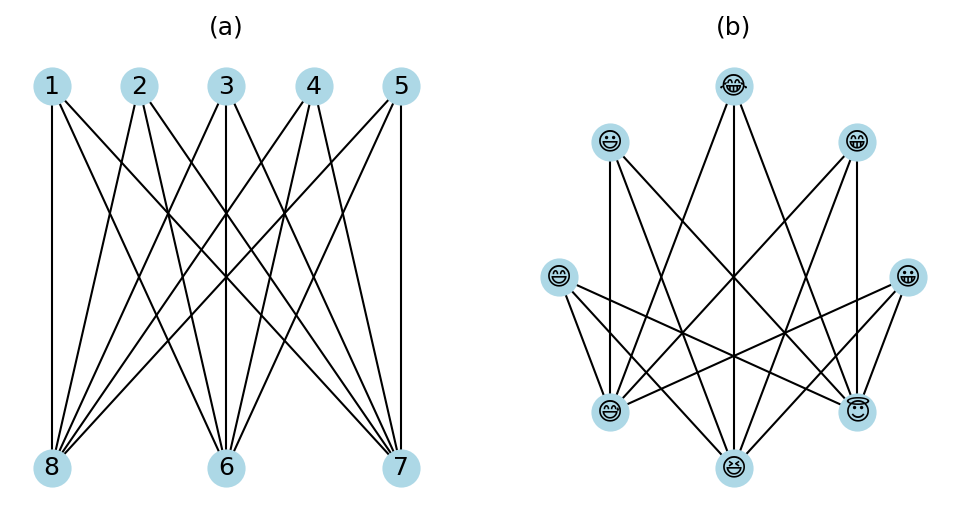
\includegraphics[scale=0.7]{figures/g-002.png}
    \caption{Both (a) and (b) are $K_{5,3}$.}
    \label{fig:2}
\end{figure}

\begin{proposition}
    Let $G[X, Y]$ and $H[U, V]$ be two complete bipartite graphs with $\abs{X} = \abs{U}$ and $\abs{Y} = \abs{V}$. Then $G \cong H$. In other words, a complete bipartite graph is unique up to isomorphism if the sizes of its two vertex sets in bipartition are determined.
\end{proposition}

\begin{proof}
    Since $\abs{X} = \abs{U}$ and $\abs{Y} = \abs{V}$, we can find a bijection $\theta: V(G) \to V(H)$ in such a way that $\theta$ maps each point in $X$ onto $U$, and each point in $Y$ onto $V$. Then for an edge $xy \in E(G)$, we have $\theta(x)\theta(y) \in E(H)$ since there has to be an edge connecting $\theta(x) \in U$ and $\theta(y) \in V$ by the definition of complete bipartite graphs. This proves $G \cong H$ by Proposition~\ref{pro:1}.
\end{proof}


%------------------------------

\section{Vertex Degrees}

%------------------------------

\begin{theorem} \label{thm:5}
	The sum of degrees of all vertices
	is twice the number of edges in any graph.
	That is, 
	\begin{align*}
		\sum_{v \in V} \deg(v) = 2 \abs{E}
	\end{align*}
\end{theorem}

\begin{proof}
	% TODO
\end{proof}

\begin{corollary} \label{cor:2}
	The number of vertices of odd degree is even
	in any graph.
\end{corollary}

%------------------------------

\section{Graph Realization Problem}

%------------------------------

Let $G$ be a graph with vertices $v_1, \ldots, v_n$.
The \textbf{degree sequence}\index{degree sequence} of $G$, 
as the name suggests,
is a list of integers consists of vertex degrees.
It is denoted by 
\begin{align*}
	\mathbf{d} = (\deg(v_1), \ldots, \deg(v_n))
\end{align*}
And it is often written in decreasing order.

Given an arbitrary list of non-negative integers
$\mathbf{d}^\prime = (d_1^\prime, \ldots, d_n^\prime)$,
it is possible that 
we cannot find any graphs whose degree sequence
is $\mathbf{d}^\prime$.
For example, no graphs have the following degree sequence:
\begin{align*}
	(2, 2, 1, 1, 1)
\end{align*}
Why? Note that $2+2+2+1+1+1 = 9$.
Hence, by Theorem~\ref{thm:5}, we see that is is impossible to 
find such a graph since the sum of degrees should be an even number.
Alternatively, one may also argue by Corollary~\ref{cor:2}
that the number of odd vertices (the last three vertices)
is 3, which is an odd number.

So, what conditions must a list of non-negative integers
must satisfy so that it is a degree sequence?
The answer is simple,
as the next proposition will show,
the provided list of integers only need to satisfy 
condition given in Theorem~\ref{thm:5}, that is, 
all the integers need to sum up to an even number. 

\begin{proposition} \label{pro:10}
	A sequence $(d_1, \ldots, d_n)$ of non-negative integers
	is a degree sequence if and only if 
	$\sum_{i=1}^n d_i$ is even.
\end{proposition}

\begin{proof}
	% TODO
\end{proof}

From the above proof, we see that
the graph we construct is a multigraph
since we mainly increase the vertex degrees by adding loops.
This invites us to think can we 
construct a \textit{simple graph}
out of the given sequence of integers?
This question is much more complecated.
And we say that a sequence of integers 
is \textbf{graphical}\index{graphical degree sequence}
if it is a degree sequence of some simple graph.
The problem of finding such a simple graph
is referred to as 
the \textbf{graph realization problem}\index{graph realization problem}.

%------------------------------

\subsection{Havel-Hakimi Theorem}

The algorithm \parencite{hakimiRealizabilitySetIntegers1962}
constructs a simple graph 
through a recursive procedure.
The theorem it based on is referred to 
as Havel-Hakimi theorem.
Before proving this theorem, 
we first introduce a lemma, 
which will be helpful in the later proof.

\begin{lemma} \label{lem:2}
	Let $G$ be a simple graph.
	If
	\begin{enumerate}
		\item $u_1 v_1, u_2 v_2 \in E$ and 
		\item $u_1 v_2, u_2 v_1 \notin E$,
	\end{enumerate}
	then all vertex degrees in the graph
	\begin{align*}
		G^\prime = G - \{u_1 v_1, u_2 v_2\}
		+ \{u_1 v_2, u_2 v_1\}
	\end{align*}
	remain unchanged.
	Of course,
	$G^\prime$ has the same degree sequence as $G$.
\end{lemma}

This lemma mainly says we can move two 
non-incident edges in $G$ in a way that 
the degree sequence remains unchanged.
Refer to Figure~\ref{fig:7} to get more insight.

\begin{figure}[ht]
	\centering
	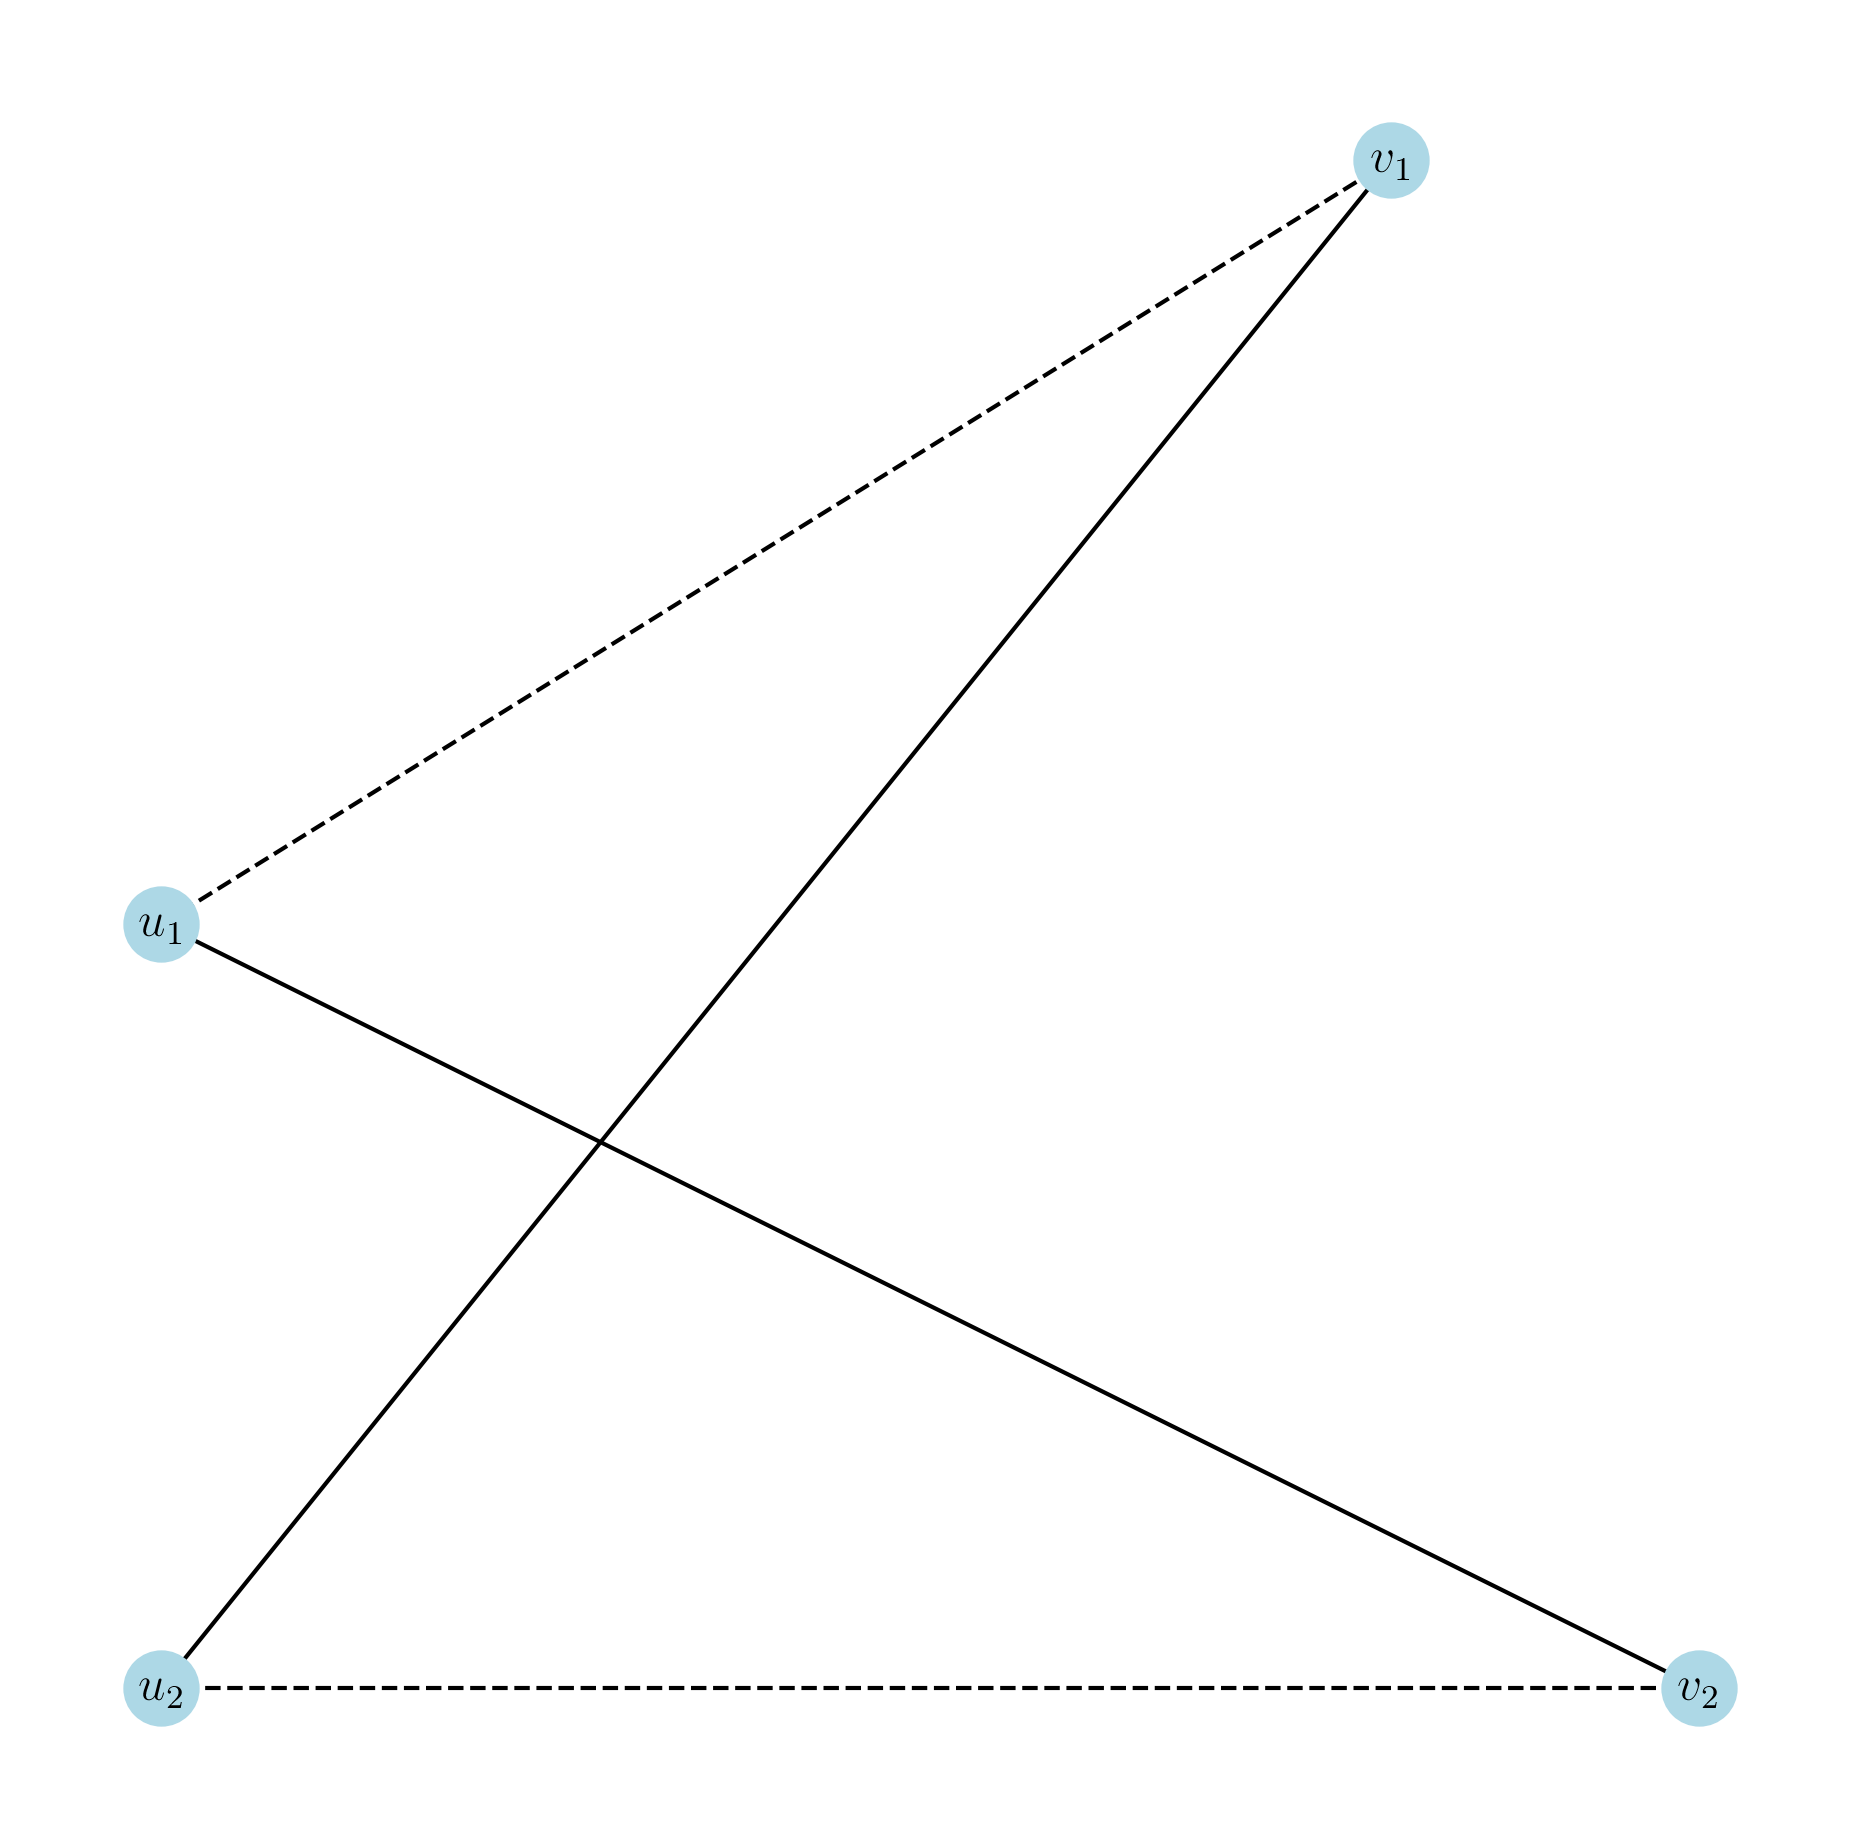
\includegraphics[scale=0.5]{figures/g-007.png}
	\caption{
		Dash lines are removed edges while
		solid lines are newly added.
	}
	\label{fig:7}
\end{figure}

\begin{proof}
	This result is evident. 
	We note that the degrees of vertices 
	$u_1$, $v_1$, $u_2$ and $v_2$ remain unchanged
	in $G^\prime$ since from the perspective of 
	each of these four vertices,
	one incident edge is removed but a new one is added.
	And the degrees of all the other vertices in $G^\prime$
	are also the same as in $G$.
\end{proof}

%------------------------------

We now present 
the \textbf{Havel-Hakimi theorem}\index{Havel-Hakimi theorem}.

\begin{theorem}[Havel-Hakimi] \label{thm:8}
	Let $\mathbf{d}=(d_1, \ldots, d_n)$
	be a decreasing sequence of non-negative integers. 
	Define $\mathbf{d}^\prime$ as 
	\begin{align*}
		\mathbf{d}^\prime
		= ( \underbrace{
			d_2 - 1, \ldots, d_{d_1 + 1} - 1
		}_{\text{$d_1$ terms}}, d_{d_1 + 2}, \ldots, d_n )
	\end{align*}
	Then $\mathbf{d}$ is graphical 
	if and only if $\mathbf{d}^\prime$ is graphical.
\end{theorem}

\begin{algorithm}[ht] 
	\caption{
		Reconnecting Graph Edges in 
		Proving Havel-Hakimi Theorem
	}
	\label{alg:5}
	\KwIn{
		A sequence of non-negative 
		integers $d_1, \ldots, d_n$
		satisfying $d_1 \geq \cdots \geq d_n$.
		A simple graph $G$ on $n$ vertices
		with $\deg(v_1) = d_1, \ldots, \deg(v_n) = d_n$.
	}
	\KwOut{
		A graph whose vertex degrees remain unchanged and
		$v_1 v_2, \ldots, v_1 v_{d_1 + 1} \in E$.
	}
	\For{$j = 2, \ldots, d_1 + 1$}{
		\If{$v_1 v_j \in E$}{
			\Continue \;
		}
		\tcp{now we have $v_1 v_j \notin E$}
		pick $u \in V \setminus \{v_2, \ldots, v_{d_1 + 1}\}$ 
		s.t. $v_1 u \in E$ \;
		pick $w \in N(v_j)$ 
		s.t. $u w \notin E$ \;
		remove edges $v_1 u$ and $v_j w$ \; 
		connect edges $v_1 v_j$ and $u w$ \;
	}	
\end{algorithm}

\begin{proof}
	($\impliedby$) 
	Let $G^\prime$ be a simple graph with 
	degree sequence $\mathbf{d}^\prime$.
	Suppose $V(G^\prime) = v_2, \ldots, v_n$ and 
	\begin{align*}
		\deg(v_2) = d_2 - 1, \; \ldots, \;
		\deg(v_{d_1 + 1}) = d_{d_1 + 1} - 1, \;
		\deg(v_{d_1 + 2}) = d_{d_1 + 2}, \; \ldots, \;
		\deg(v_n) = d_n
	\end{align*}
	Now, find a vertex, say $v_1$, that is distinct from 
	the existing vertices of $G^\prime$,
	and then join $v_1$ with $v_2, \ldots, v_{d_1 + 1}$.
	We call the resulting graph $G$.
	Observe that $\deg(v_1) = d_1$ and 
	the degrees of $v_2, \ldots, v_{d_1 + 1}$ are all increased by one.
	Hence, the degree sequence of $G$ is exactly $\mathbf{d}$.

	($\implies$)
	Suppose that $G$ is a graph with degree sequence $\mathbf{d}$
	and that
	\begin{align*}
		\deg(v_1) = d_1, \; \ldots, \; \deg(v_n) = d_n
	\end{align*}
	\begin{note}
		The difficulty of proving this direction is 
		that $v_1$ is not necessarily
		to be incident with	$v_2, \ldots, v_{d_1 + 1}$.
		So, we need to design an algorithm to 
		alter the original graph without 
		changing its degree sequence 
		so that $v_1$ is incident with $v_2, \ldots, v_{d_1 + 1}$.
		See Algorithm~\ref{alg:5}.
	\end{note}
	\noindent In the following, we prove the correctness 
	of Algorithm~\ref{alg:5}.

	\noindent\textbf{Loop Invariants:}
	Upon completion of iteration $j$, we have 
	\begin{enumerate}
		\item All vertex degrees remain the same, and 
		\item $v_1 v_2, \ldots, v_1 v_j \in E$.
	\end{enumerate}
	(Note that there is no need to prove the initialization part
	of this algorithm.)

	\noindent\textbf{Maintenance:}
	If the condition in line 2 is satisfied,
	then the loop invariant holds.
	Now, suppose that $v_1 v_j \notin E$.

	We first show why line 5 works.
	Assume we cannot find such vertex $u$,
	which means $v_1$ is not incident with any vertex 
	other than $\{v_2, \ldots, v_{d_1 + 1}\}$.
	Because $v_1$ is incident with $d_1$ vertices,
	it must be incident with all vertices 
	in $\{v_2, \ldots, v_{d_1 + 1}\}$,
	which leads to a contradiction since $v_1 v_j \notin E$.
	Hence, we can always find such a $u$ specified by line 5.

	Let us now prove the correctness of line 6.
	Assume, on the contrary,
	there is no such vertex $w$.
	Then $u$ is incident with every neighbor of $v_j$,
	which implies that 
	\begin{align*}
		\deg{u} \geq \deg(v_j)
	\end{align*}
	Moreover, $u$ is also incident with $v_1$ whereas $v_j$ is not.
	Hence, 
	\begin{align*}
		\deg{u} > \deg(v_j)
	\end{align*}
	But the degree of $u$ should be less than or equal to 
	that of $v_j$ based on the given condition.
	Hence, this leads to a contradiction and 
	line 6 also works.

	Since $v_1 u, w v_j \in E$ and $v_1 v_j, w u \notin E$,
	by applying Lemma~\ref{lem:2},
	we know that all vertex degrees remain unchanged
	after executing line 7 and line 8.
	(Note that now $v_1 v_j \in E$.)
	This proves the loop invariants.

	\noindent\textbf{Termination:}
	Upon termination, the result is as desired
	due to the loop invariants.

	Now, by removing vertex $v_1$,
	we will reduce the degree of $v_2, \ldots, v_{d_1 + 1}$ by one.
	Hence, $G^\prime = G - v_1$ has the 
	degree sequence $\mathbf{d}^\prime$, and 
	it is of course simple.
	Therefore, $\mathbf{d}^\prime$ is graphical.
\end{proof}

%------------------------------

\section{Paths and Connection}

%------------------------------

A \textbf{walk}\index{walk in a graph} in a graph is a sequence of edges $e_1 \cdots e_k$ joining a \textit{nonempty} sequence of vertices $v_0 v_1 \cdots v_k$, which is denoted by 
\begin{align}
    v_0 e_1 v_1 \cdots e_k v_k 
    \label{eq:3}
\end{align}
with each edge written after one of its end and followed by its other end. Note that though the sequence of vertices in a walk is required to be nonempty, the sequence of edges may be empty. And in that case, the walk contains only one vertex, say $v_0$, and it is called the \textbf{trivial walk}\index{trivial walk}.
\begin{note}
    The term \textbf{sequence} in mathematics often means an infinite sequence, which is essentially a function defined on $\N^\ast$. However, in graph theory, we usually refer to sequence as a \textbf{finite} list of ordered elements.
\end{note}

We call a walk $W$ from $v_0$ to $v_k$ a $(v_0, v_k)$-walk. The vertices $v_0$ and $v_k$ are referred to as the \textbf{origin}\index{origin of a walk} and the \textbf{terminus}\index{terminus of a walk} of that walk, respectively. 

It should be emphasized that neither the edges nor the vertices in a walk are necessarily distinct. However, if all edges of walk $W$ are distinct, we call $W$ a \textbf{trail}\index{trail in a graph}. And if all vertices in $W$ are distinct, it is then called a \textbf{path}\index{path in a graph}. Of course, all edges in a path are also distinct since the vertices are.

Two vertices are said to be \textbf{connected}\index{connected and disconnected vertices} if there exists a path joining them. Otherwise, they are \textbf{disconnected}. 

The length of a path $P$, written as $\abs{P}$, is defined as the number of edges along it. Note that the length of a trivial path is zero since there are no edges.

If $G$ is a simple graph, then we may write a walk simply as a sequence of vertices since there is one and only one edge joining each pair of consecutive vertices in the walk. For example, we write the $(v_0, v_k)$-walk in \eqref{eq:3} as 
\begin{align*}
    v_0 v_1 \cdots v_k
\end{align*}
with edges dropped.

%------------------------------

\begin{proposition} \label{pro:7}
    If there is a $(u, v)$-walk in $G$, then there is also a $(u, v)$-path in $G$.
\end{proposition}

This can be proved easily using the following algorithm (Algorithm~\ref{alg:1}).

\begin{algorithm}[ht]
    \KwIn{A walk $W = v_0 e_1 v_1 \cdots e_k v_k$}
    \KwOut{A path $P$}
    initialize $P$ as a sequence containing just one vertex $v_0$ \;
    \For{$i = 1, \ldots, k$}{
        \eIf{$v_i$ is not in $P$}{
            append $e_i$ and $v_i$ to $P$ \;
        }{
            remove all the vertices and edges after the vertex $v_i$ from $P$ \;
        }
    }
    \caption{Extracting a Path From a Walk}
    \label{alg:1}
\end{algorithm}

%------------------------------

\begin{proposition}
    The number $(v_i, v_j)$-walks of length $k$ in $G$ is the $(i,j)$-th entry of the $k$-th power of the adjacency matrix $A$, i.e., $A^k$.
\end{proposition}

\begin{proof}
    % TODO
\end{proof}

%------------------------------

Imagine removing one edge from the original graph $G$.
Then we can obtain at most one more component 
by cutting in half one of $G$'s components.
See Figure~\ref{fig:5}.

To prove this, we first consider
the following useful lemma.

\begin{lemma} \label{lem:1}
	Let $G$ be a connected graph, 
	and $e$ be one of its edges.
	Suppose that the two ends of $e$ are $x$ and $y$.
	Then every vertex $v$ is either connected to $x$
	or $y$ in $G-e$.
\end{lemma}

\begin{proof}
	First, suppose that $e$ is a loop.
	Since $G$ is connected, 
	every two vertices are connected by a path.
	And they remain connected in $G-e$ 
	since a path cannot contain any loops.
	Hence, in this case, every vertex $v$ 
	is connected to both $x$ and $y$ in $G-e$.

	Assume $e$ is not a loop. 
	If vertex $v$ is no longer connected to $x$ in $G-e$,
	then $v$ must be originally connected to $x$
	in $G$
	by a path $P$ containing the edge $e$.
	Note that $P$ is of the form 
	\begin{align*}
		P = v \cdots y e x
	\end{align*}
	Because the $(v,y)$-section of $P$ does not traverse $e$,
	$v$ is connected to $y$ in $G-e$ by this $(v,y)$-section.
	Hence, we have shown that, 
	in subgraph $G-e$, 
	$v$ must be connected to $y$ 
	if it is disconnected from $x$.
	This completes the proof.
\end{proof}

\begin{figure}[ht]
    \centering
    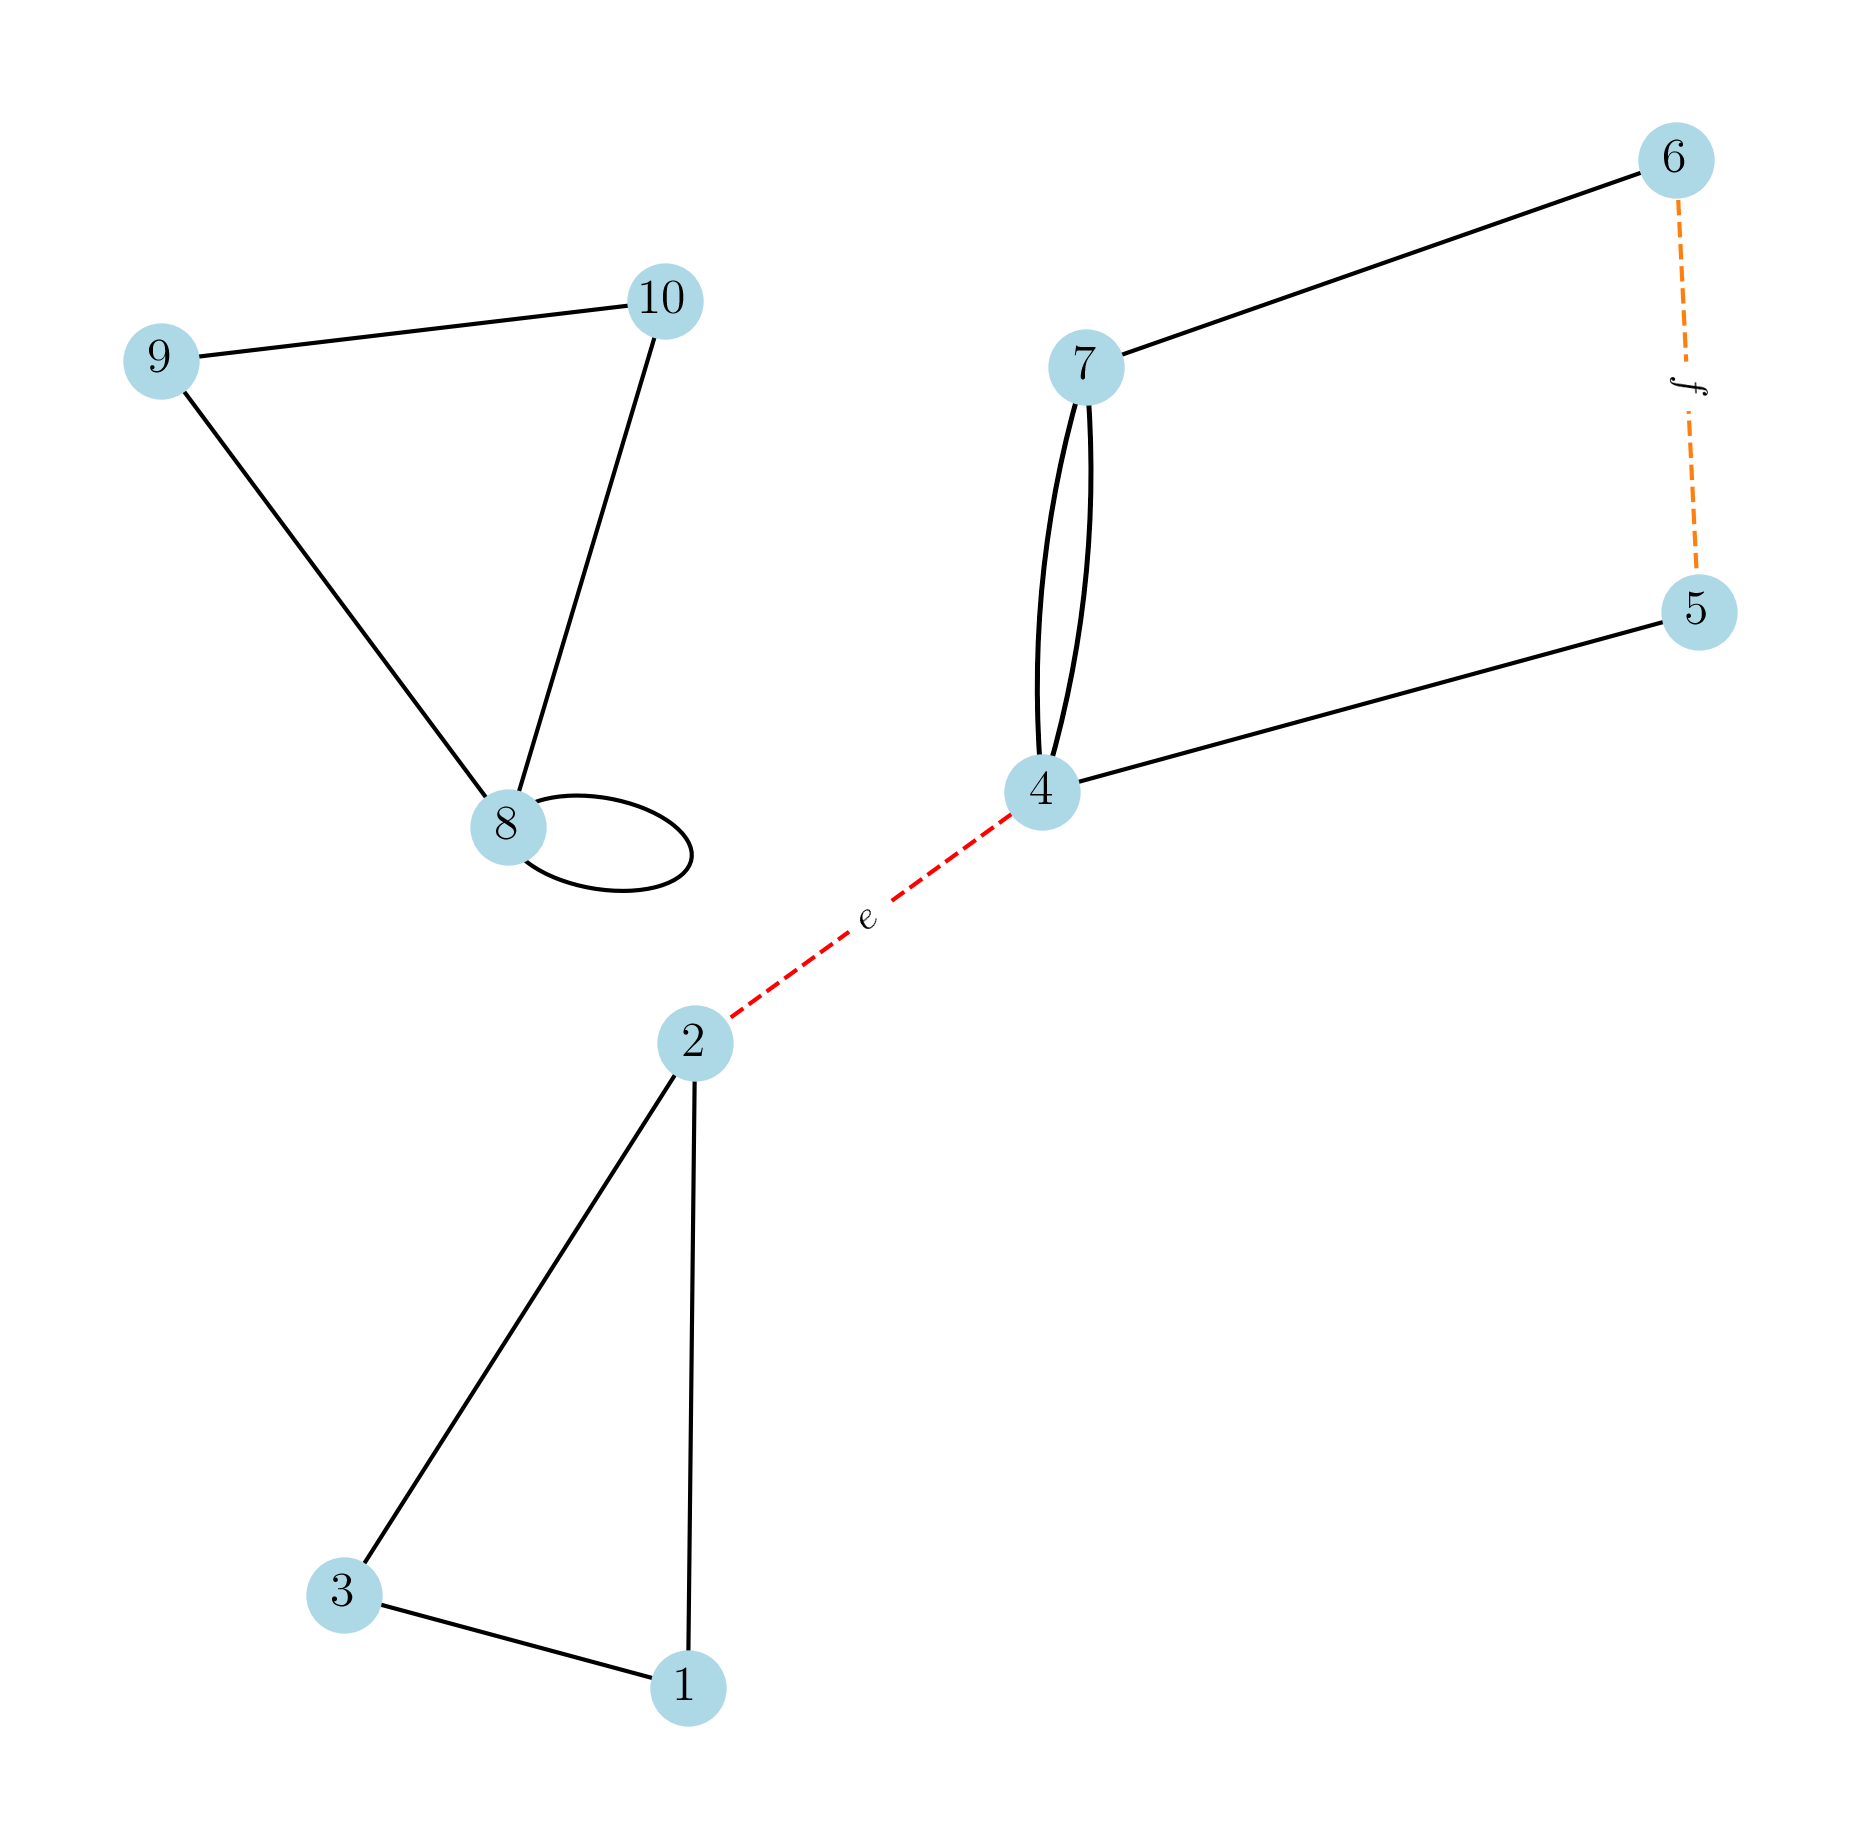
\includegraphics[scale=0.5]{figures/g-005.png}
    \caption{
		The graph $G$ has 2 components.
		If we remove edge $f$, 
		then $G-f$ still has 2 components.
		But if we remove edge $e$, then 
		the remaining graph $G-e$ has 3 components.
	}
    \label{fig:5}
\end{figure}

\begin{proposition}\label{pro:6}
    If $e \in E$, then we have 
	\begin{align}
		\omega(G) \leq \omega(G-e)
		\leq \omega(G) + 1 
		\label{eq:11}
	\end{align}
\end{proposition}

Inequalities \eqref{eq:11} describe the result 
of cutting an edge in a compact way.
The first inequality $\omega(G) \leq \omega(G-e)$
says the number of components may increase by cutting an edge.
While the second inequality says this number will be increased 
by at most one.

\begin{proof}
	If $e$ is a loop, then the conclusion is trivial. 
	We assume $e = xy$ is not a loop, i.e., 
	$x$ and  $y$ are distinct,
	in the rest of the proof. 
	Suppose that the components of $G$
	are  $G[V_1], \ldots, G[V_\omega]$.
	Without loss of generality, 
	we may also assume that $x, y \in V_1$.

	(Case 1) Suppose that there exists a $(x,y)$-path in $G-e$,
	then $x$ is still connected to $y$ in $G-e$,
	i.e., $x \sim y$ in $G-e$.
	Pick an arbitrary vertex $v \in V_1$.
	By Lemma~\ref{lem:1}, 
	we know either $v \sim x$ or $v \sim y$.
	Either way, by the transitivity, we have $v \sim x$
	since $x \sim y$. 
	Therefore, 
	\begin{align*}
		v \sim x 
		\quad \forall v \in V_1
	\end{align*}
	This means $V_1$ remains a equivalent class in $G-e$.
	In this case, $\omega(G-e) = \omega(G)$.

	(Case 2) We now consider the case where 
	$x$ is disconnected from $y$ in $G-e$.
	For any vertex $v \in V_1$,
	by Lemma~\ref{lem:1},
	we have either $v \sim x$ or $v \sim y$. 
	But $v$ cannot be connected to both $x$ and $y$
	since $x$ and $y$ are 
	assumed disconnected from each other.
	It then follows that $V_1$ can be partitioned into
	two equivalent classes, $[x]$ and $[y]$. 
	In other words, $V_1$ is split into two components in $G-e$.
	Therefore, $G-e$ has one more component than that of $G$, 
	and hence $\omega(G-e) = \omega(G) + 1$.
\end{proof}

The idea of cutting an edge 
is quite helpful in many proofs
since by doing so, 
we will probably divide the original graph 
into two smaller ones.

The edge if removed will indeed results in 
one more component deserves a name, 
as we shall define in the following.

\begin{definition} \label{def:1}
	The edge $e$ of $G$ is 
	called a \textbf{cut edge}\index{cut edge} if 
	\begin{align}
		\omega(G-e) = \omega(G) + 1
		\label{eq:14}
	\end{align}
\end{definition}

In Figure~\ref{fig:5}, $e$ is a cut edge of $G$ but $f$ is not.

\begin{note}
	Equation \eqref{eq:14}
	is replaced by 
	$\omega(G-e) > \omega(G)$ in
	\parencite{bondyGraphTheoryApplications1976}.
	But since we have already proved Proposition~\ref{pro:6}, 
	we can be more specific.
\end{note}

%------------------------------

Consider a path graph $P_n$ on $n$ vertices.
It is connected and it has altogether $n-1$ edges. 
Apparently, if we remove any edge from it, 
then we will end up with a disconnected graph.
This somehow tells us that 
for a graph to be connected,
it cannot have too few edges, 
which leads to the question that 
what is the minimum number of edges 
of a connected graph of order $n$?

\begin{proposition} \label{pro:8}
	The minimum number of edges of 
	a connected graph on $n$ vertices
	is $n-1$.
\end{proposition}

\begin{proof}
	We shall prove by induction on the order.
	The induction hypothesis is that
	if $G$ is a connected graph $G$ with minimum number of edges
	and its order is less than or equal to $n$,
	then it has exactly $n-1$ edges.

	\noindent\textbf{Base Case:} 
	If $G$ is a trivial graph, 
	then clearly it has no edges.

	\noindent\textbf{Inductive Step:}
	Assume the hypothesis holds for $n = k$.
	Note that we only need to show 
	$G$ has $k$ edges under the case where 
	$G$ is of order $k+1$.
	Because $G$ is a connected graph with minimum number
	of edges.
	By removing any edge, say $e$, from $G$ 
	will result in a disconnected graph $G-e$.
	And by Proposition~\ref{pro:6}, 
	we know $G-e$ has two components, say $G_1$ and $G_2$.
	Note that both $G_1$ and $G_2$ are of 
	orders less than or equal to $k$, 
	say $n_1$ and $n_2$, respectively.
	Moreover, both $G_1$ and $G_2$ are connected graphs
	with minimum number of edges.
	Hence, applying the induction hypothesis 
	to both $G_1$ and $G_2$,
	we conclude that 
	\begin{align*}
		\abs{E(G_1)} = n_1 - 1 
		\quad \text{and} \quad 
		\abs{E(G_2)} = n_2 - 1
	\end{align*}
	Therefore, the total number of edges of $G$ is 
	\begin{align*}
		\abs{E(G)} = \abs{E(G_1)} + \abs{E(G_2)} + 1 
		= n_1 - 1 + n_2 - 1 + 1 
		= n_1 + n_2 - 1
		= \abs{V(G)} - 1
		= k
	\end{align*}
	The second last equality follows from the fact that 
	the vertices of $G$ is partitioned into 
	vertices of $G_1$ and $G_2$, respectively,
	since $G_1$ and $G_2$ are complements.
	This completes the proof.
\end{proof}

Apart from the path graph $P_n$, 
Figure~\ref{fig:6} also depicts several other 
connected graphs of order 6 
with minimum number of edges, 
in this case, 5 edges.
Such graphs are called trees, 
as we will formally introduce in Chapter~\ref{chap:1}.

\begin{figure}[ht]
	\centering
	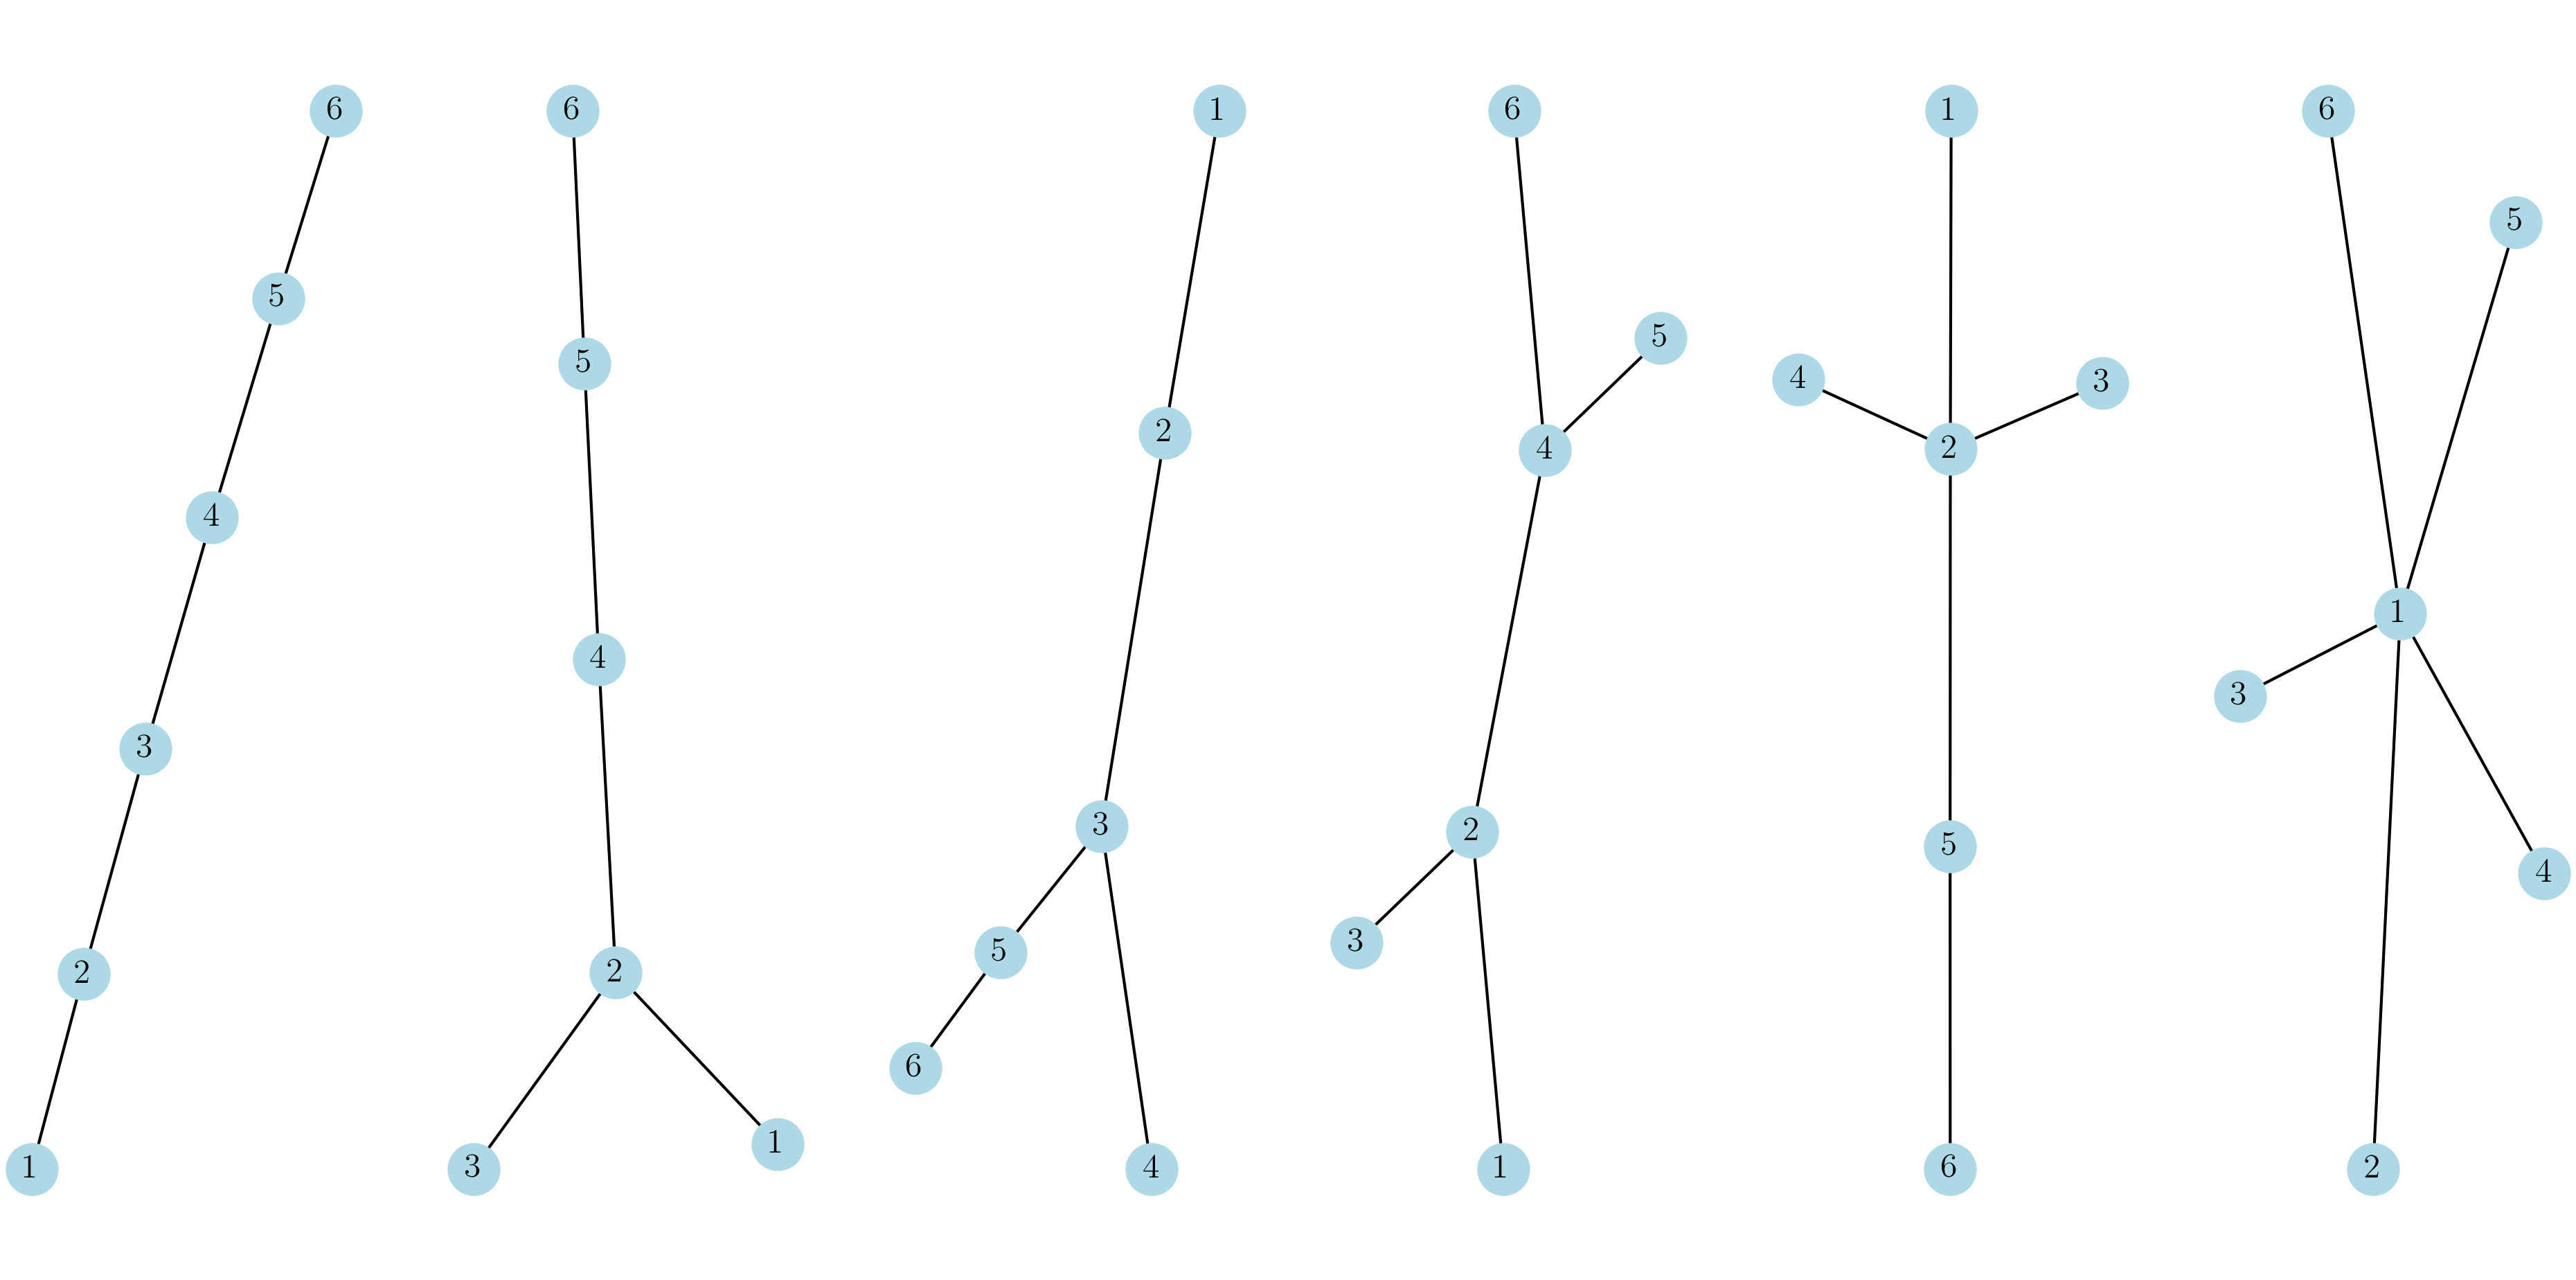
\includegraphics[scale=0.5]{figures/g-006.png}
	\caption{
		Connected graphs on 6 vertices 
		with minimum number of edges, 
		i.e., 5 edges.
	}	
	\label{fig:6}
\end{figure}


%------------------------------

\begin{proposition} \label{pro:7}
	Let $G$ be a simple and connected graph
	with order greater than or equal to 3.
	If $G$ is not complete,
	then there exist three vertices $u$, $v$ and $w$ such that 
	$uv, vw \in E$ but $uw \notin E$.
\end{proposition}

\begin{proof}
	Because $G$ is not complete, 
	there exist two vertices $u$ and $w$ that are not incident.
	Let $P$ be a shortest path from $u$ to $w$.
	
	If $P$ is of length 2, then we can write 
	$P = u v w$.
	Edges $uv$ and $vw$ exist in $G$. 
	But the edge $uw$ does not, which is as desired.

	If the length of $P$ is greater than or equal to $3$, 
	then $P$ is of the form 
	\begin{align*}
		P = u x v \cdots w 
	\end{align*}
	Note that $uv \notin E$. 
	Otherwise, $u v \cdots w$ would be 
	a shorter $(u,w)$-path than $P$.
	In this case the vertices $u$, $x$ and $v$ are as desired.
\end{proof}

%------------------------------

\section{Cycles}

%------------------------------

One simple yet useful observation of a particular longest path 
in a graph is that all the neighbors of the terminus must 
occur along the path. To be specific, 
if $P = v_0 e_1 v_1 \cdots e_k v_k$ is one of the longest paths in $G$ 
then $P$ must contain all vertices in $N(v_k)$. 
To prove this, we assume $P$ does not contain $v_{k+1} \in N(v_k)$. 
(Suppose $\psi(e_{k+1}) = v_k v_{k+1}$.) 
Then the path $P + e_{k+1}v_{k+1}$ is clearly longer than $P$, 
which leads to a contradiction. 
Figure~\ref{fig:1} depicts such an example. 
Note that if $8$ were a neighbor of $7$, 
then path $12345678$ would be longer.

\begin{figure}[ht]
    \centering
    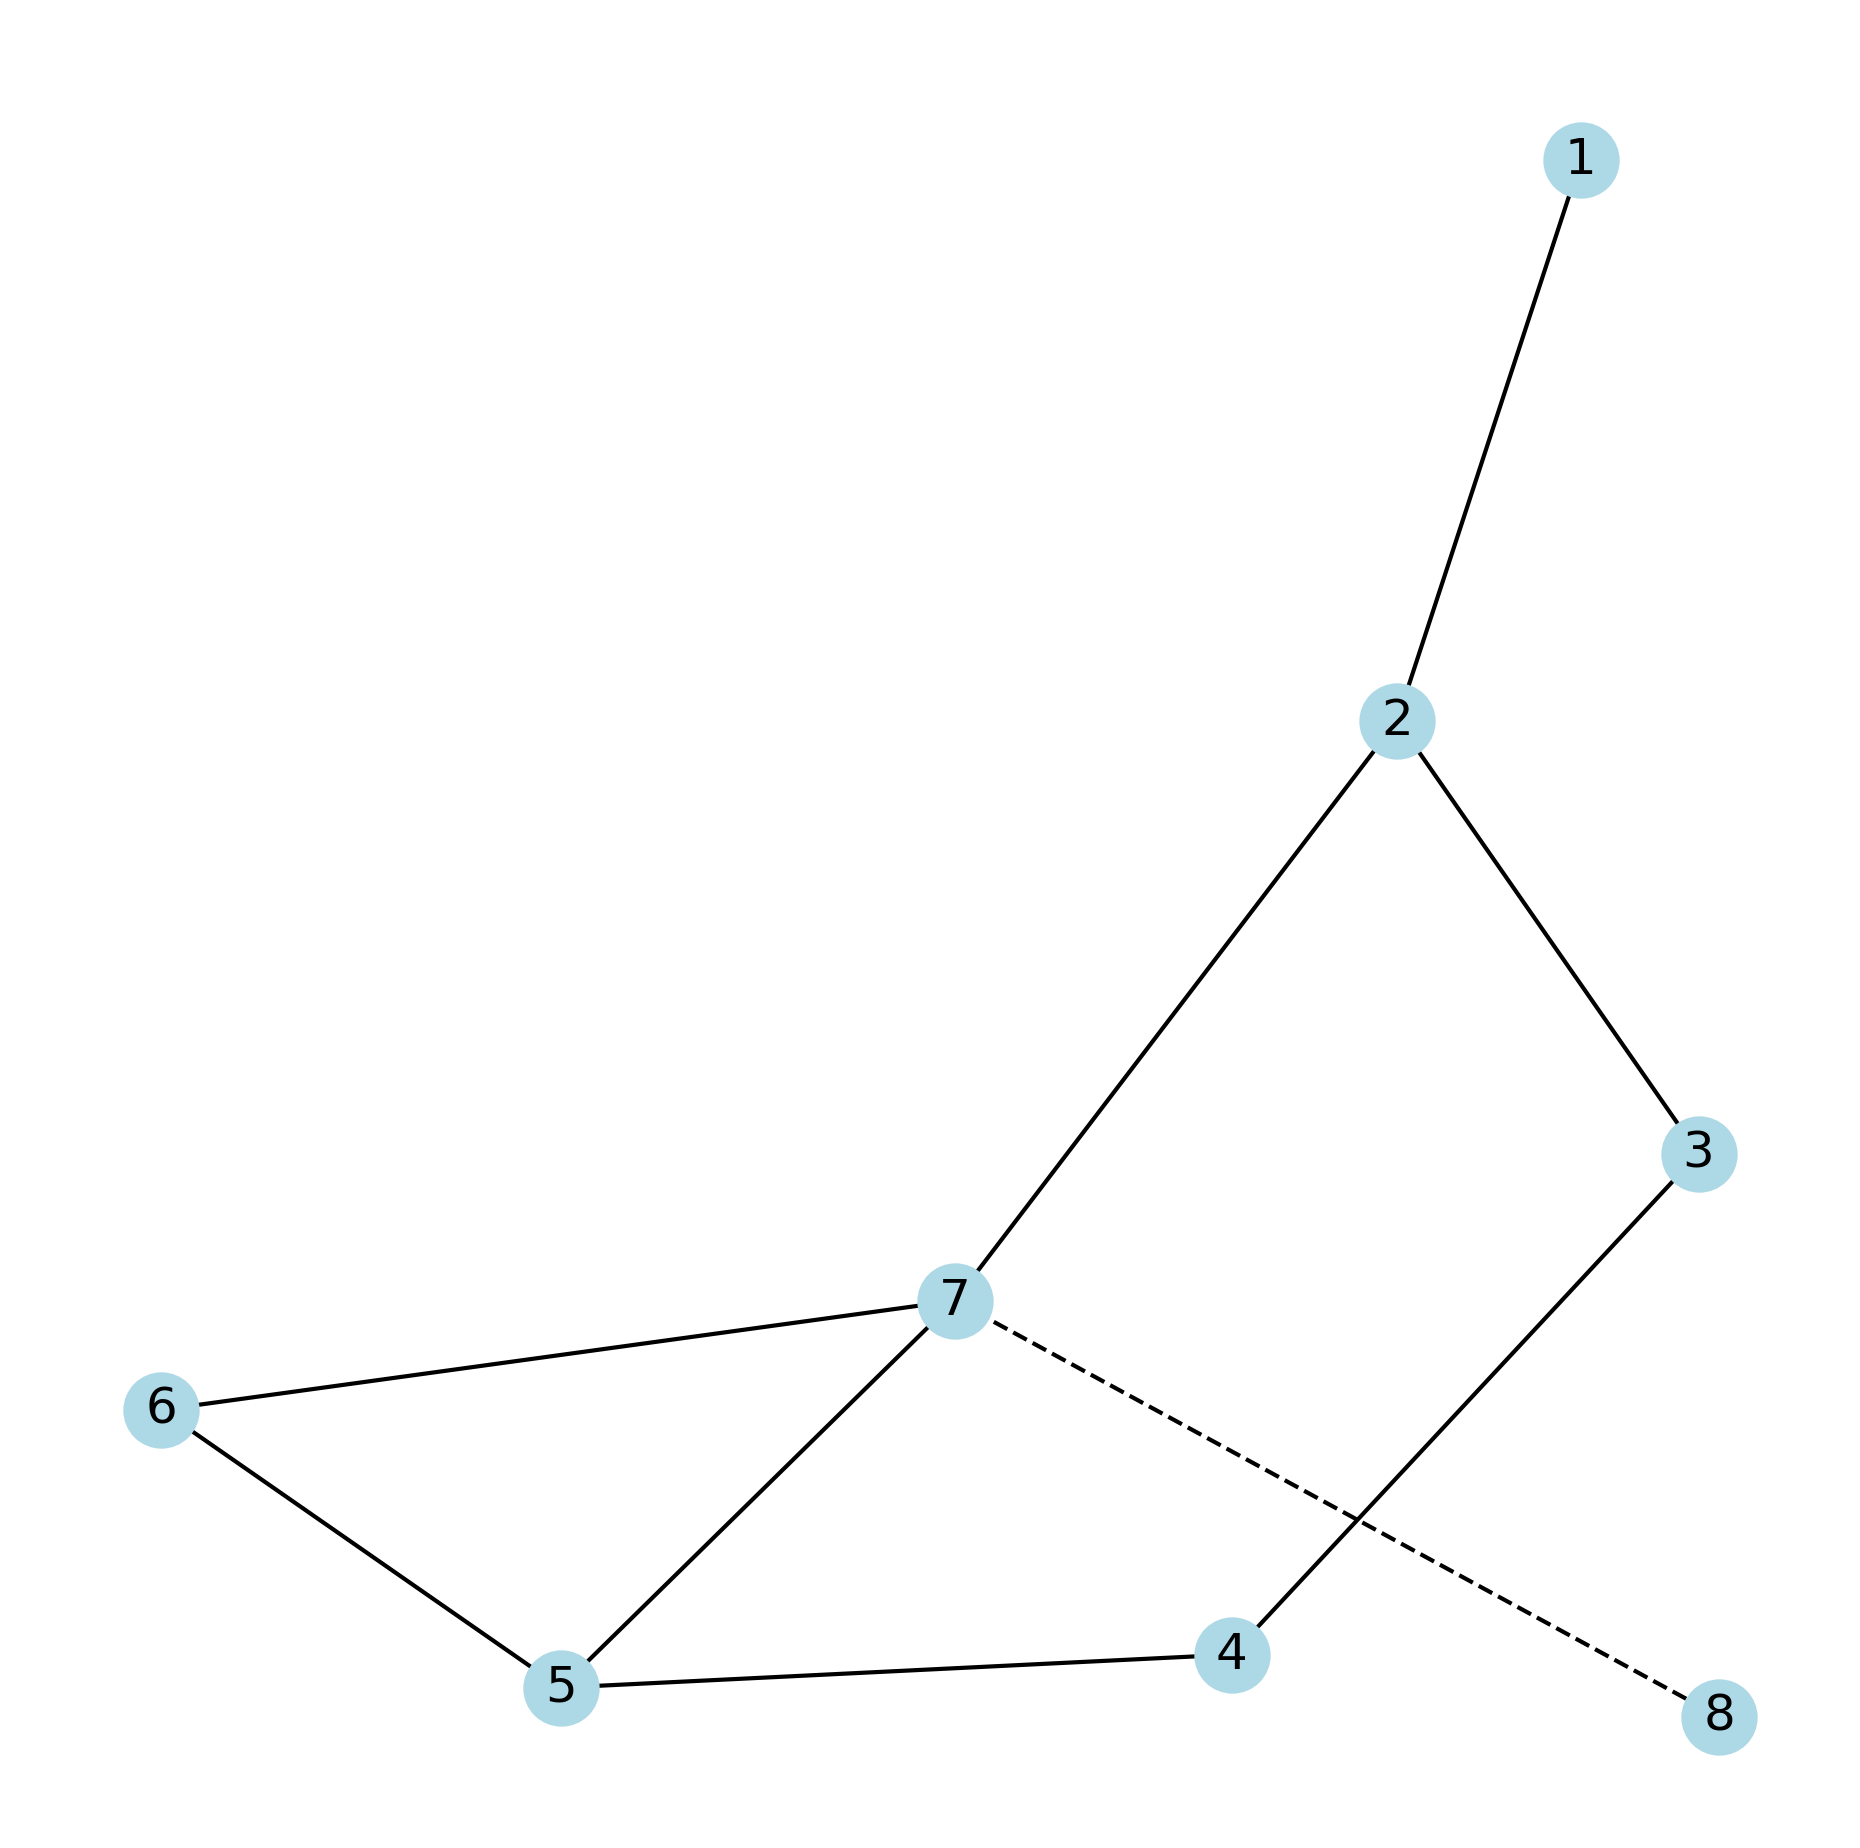
\includegraphics[scale=0.5]{figures/g-001.png}
    \caption{Path $1234567$ is one of the longest paths.}
    \label{fig:1}
\end{figure}

%------------------------------

\begin{proposition} \label{pro:5}
    If $G$ is a simple graph with $\delta(G) \geq 2$, 
	then there exists a cycle of length 
	at least $\delta(G)+1$.
\end{proposition}

\begin{proof}
	Let $P = u \cdots v$ 
	be a longest path in $G$.
	As noted before, all the neighbors of 
	the terminus $ v $,
	denoted by $v_1, \ldots, v_{\delta(G)}$
	arranged by their original order in $P$,
	must occur along the path $P$.
	Note that the $(v_1, v)$-section,
	denoted by $Q$,
	is of length $\delta(G)$.
	Because $\deg(v) \geq 2$, 
	$v$ has at least two neighbors. 
	In other words,
	the section $Q$ is different from the edge 
	connecting $v$ and $v_1$.
	Hence, $Q v_1$ forms a cycle.
	And it is of length $\delta(G) + 1$.
	This completes the proof.
\end{proof}

In fact, we have an algorithm to find a cycle without knowing the longest path in $G$.

\begin{algorithm}[ht]
    \KwIn{$G$ with $\delta(G) \geq 2$}
    \KwOut{A cycle $C$}
    \If{$G$ has a loop $e$ from $v$ to $v$}{
        $C \gets v e v$ \;
        \Return{$C$} \;
    }
    pick a vertex $v_0$ \; 
    $P \gets v_0$ \;
    pick $v \in N(v_0)$ and let $e$ be the corresponding edge, i.e., $\psi(e) = v_0 v$ \;
    \While{$v \notin P$}{
        $P \gets P e v$ \;
        pick $u \in N(v)$ such that
        there exists an edge $f$ satisfying $\psi(f) = v u$ and $f \neq e$ \;
        $v \gets u$ \; 
        $e \gets f$ \;
    }
    remove from $P$ all vertices and edges before $v$ \;
    $C \gets P e v$ \;
    \caption{Finding a Cycle in $G$ With $\delta(G) \geq 2$}
    \label{alg:2}
\end{algorithm}

\begin{proof}
We need to show that Algorithm~\ref{alg:2} works correctly. 
    
\noindent \textbf{Initialization:} Firstly, note that line 7 is possible 
since $v_0$ has no loops and $\deg(v_0) \geq 2$. 

We claim the loop invariants are
\begin{enumerate}
    \item $P$ has $j$ vertices assuming that 
		we are to execute the $j$-th iteration,
    \item $P$ has no duplicated vertices, i.e., $P$ is a path, and
    \item edge $e$ is incident with $v$.
\end{enumerate}

\noindent \textbf{Maintenance:} Suppose we are in the $j$-th iteration. 
After line 9, $P$ remains a path. Because $\deg(v) \geq 2$, 
there exists an edge $f$ other than $e$ that is incident with $v$. 
Hence, line 10 works correctly. 
After executing line 12, we find that the number of vertices in $P$ is increased by one, i.e., $j+1$, 
$P$ is still a path and $e$ is incident with $v$.

\noindent \textbf{Termination:} We can complete at most $n-1$ iterations 
since $P$ can hold at most as many vertices as there are in $G$. 
Upon termination, 
we find $v$ is in $P$ and $e$ is incident with $v$. 
By removing from $P$ all vertices and edges before $v$ 
and then append to it edge $e$ and vertex $v$, 
we will obtain a cycle from $v$ to itself. 
\end{proof}

%------------------------------



%------------------------------

\begin{theorem} \label{thm:1}
	Graph $G$ is a bipartite graph 
	if and only if 
	it contains no odd cycles.
\end{theorem}

\begin{proof}
	% TODO
\end{proof}

%------------------------------

The \textbf{girth}\index{girth} of a graph is defined as 
the length of its shortest cycle.
We say the girth of $G$ is infinity if it contains no cycles.
Apparently, if $G$ has girth 1, then it contains a loop.
If it has girth 2, then there must be a parallel edge. 
But it has no loops.
And if the girth of $G$ is greater than or equal to 3,
then it must be a simple graph.

\begin{proposition}\label{pro:3}
	A $k$-regular graph with girth 4 has at least $2k$ vertices.
	Moreover, if it has exactly  $2k$ vertices, 
	then it must be $K_{k,k}$, i.e.,
	a complete bipartite graph with both sides of 
	the bipartition having the same size $k$.
	Conversely, $K_{k,k}$ is a $k$-regular graph with girth 4.
\end{proposition}

Figure~\ref{fig:3} depicts several $K_{k,k}$ graphs.

\begin{figure}[ht]
    \centering
    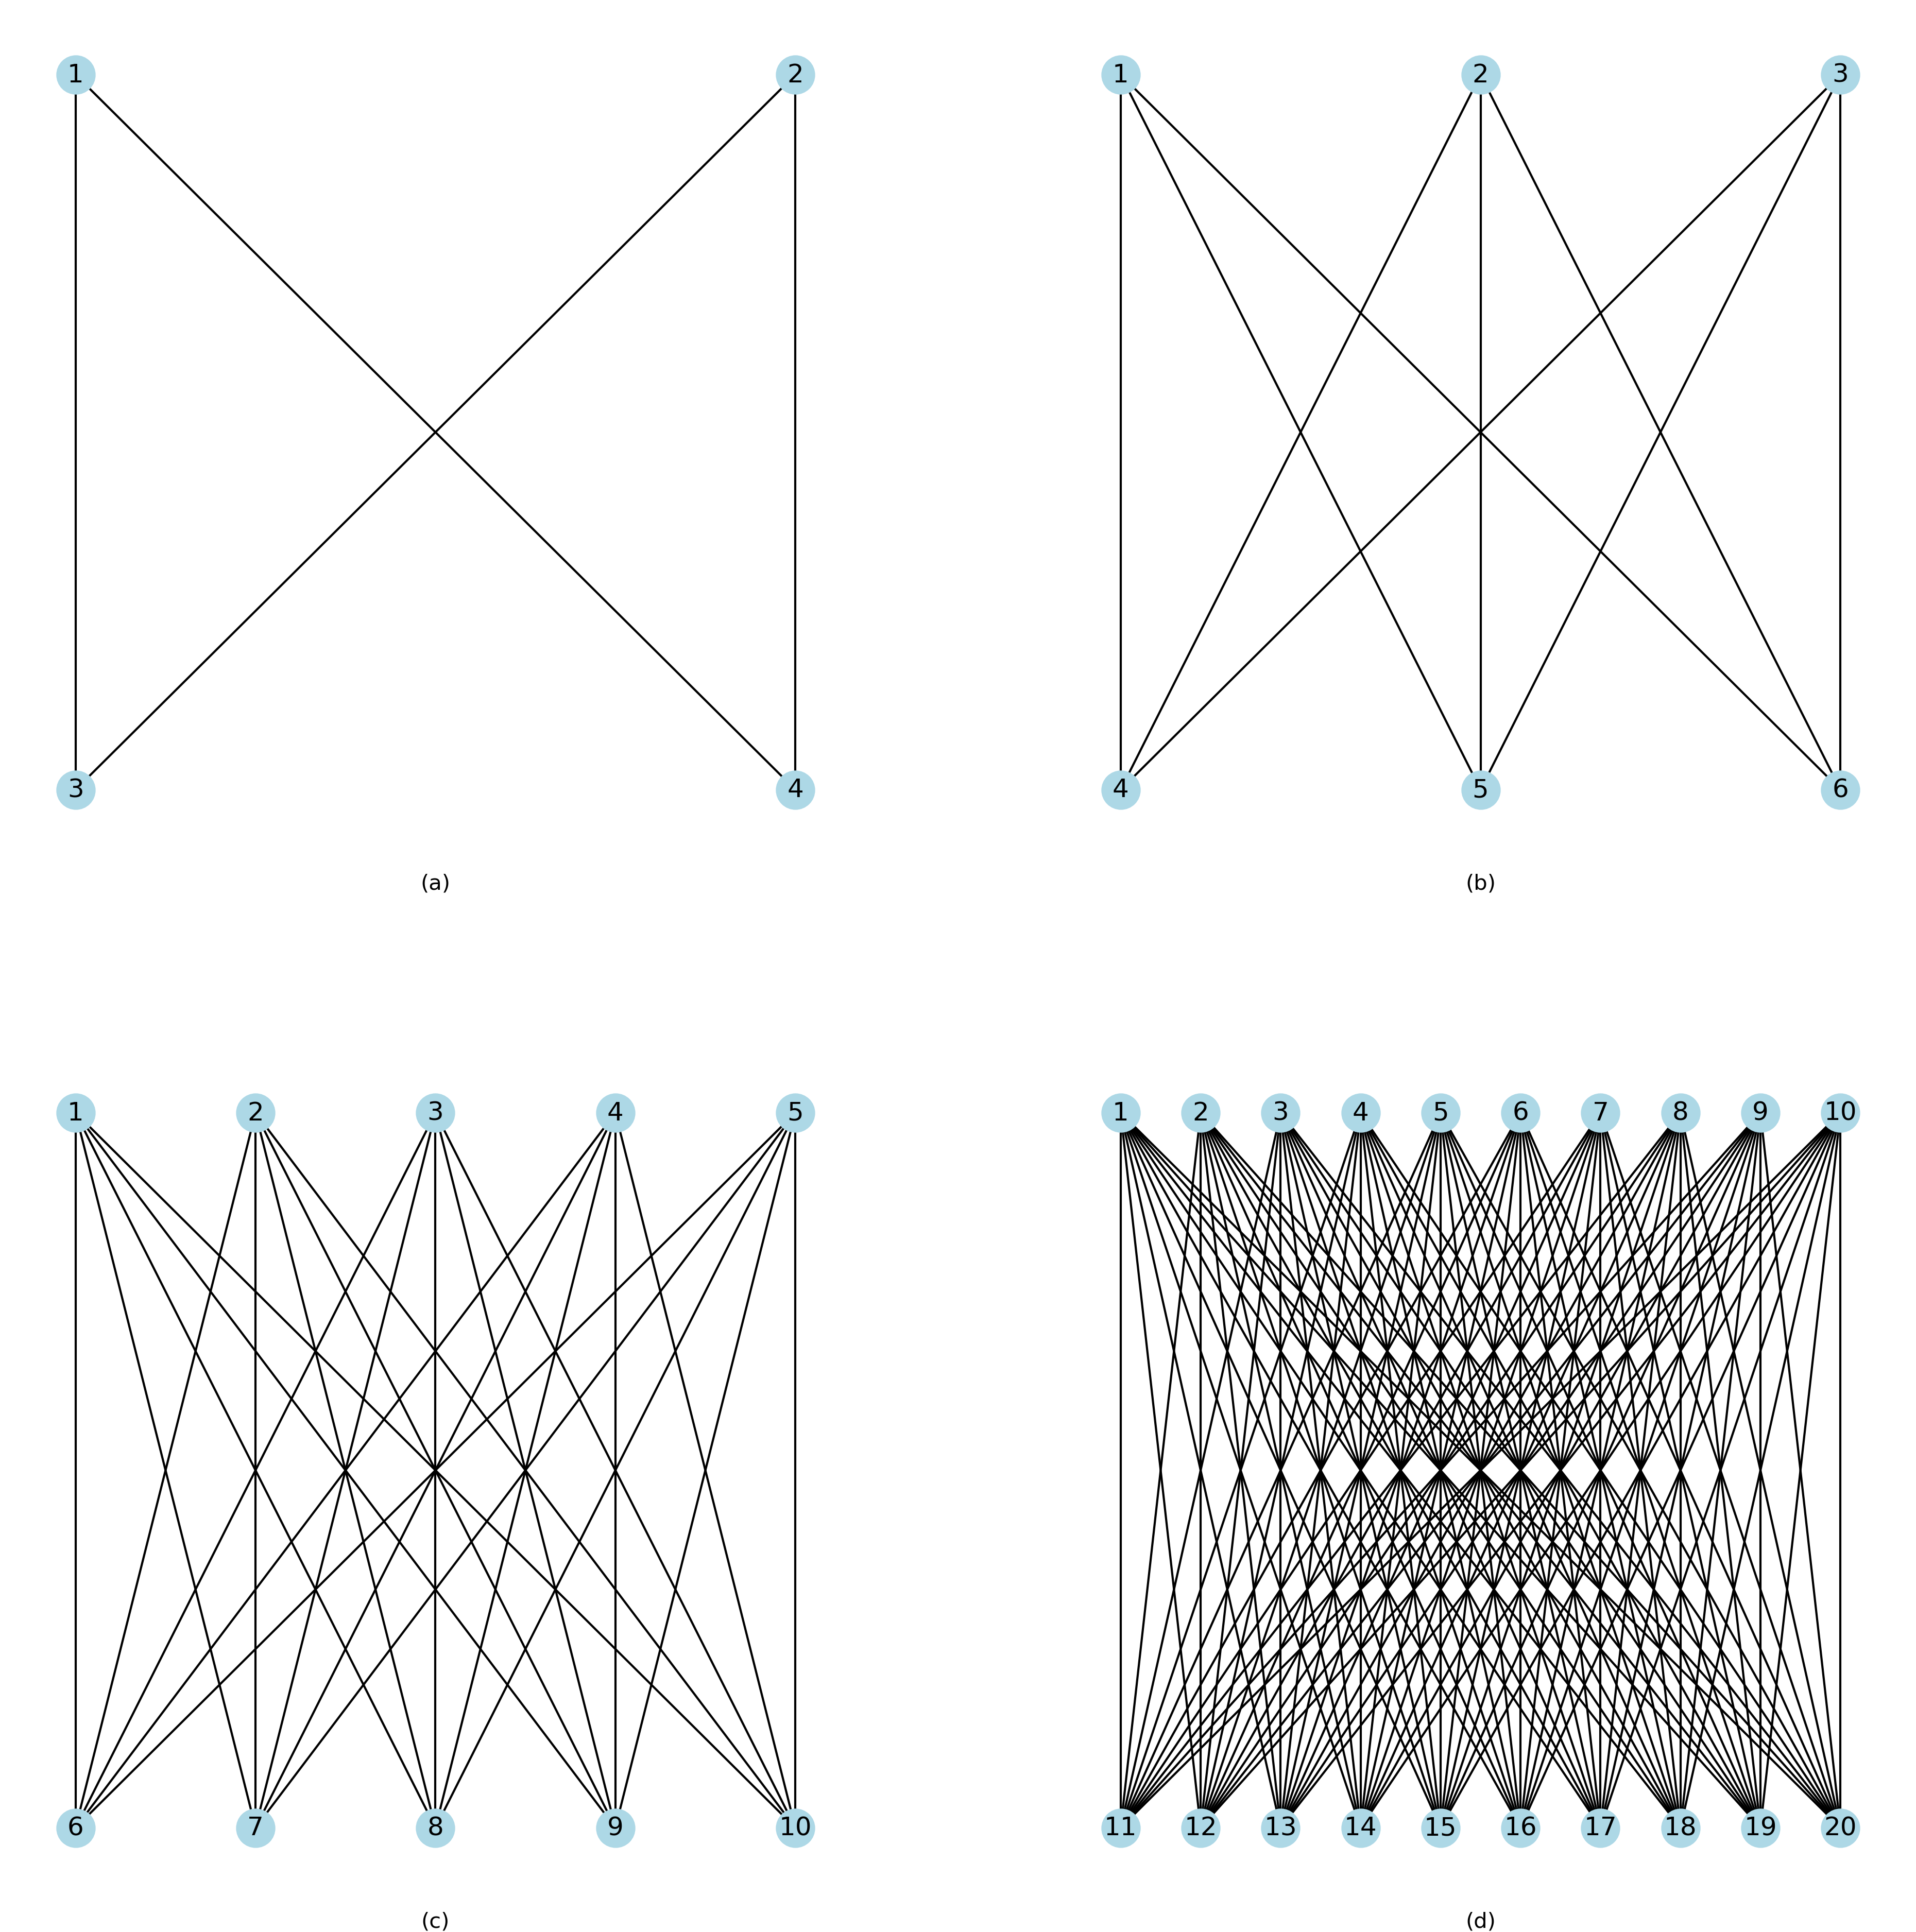
\includegraphics[scale=0.5]{figures/g-003.png}
	\caption{(a) $K_{2,2}$. (b) $K_{3,3}$. (c)  $K_{5,5}$. 
	(d)  $K_{10,10}$.}
    \label{fig:3}
\end{figure}

\begin{proof}
    Take a pair of incident vertices $u$ and $v$ in $G$.
	We have $N(u) \cap N(v) = \emptyset$. 
	Otherwise, a triangle would appear. 
	Because the degrees of $u$ and  $v$ are both $k$,
	equivalently, the sizes of their neighbors are $k$,
	$G$ must has at least $2k$ vertices 
	having these two disjoint sets $N(u)$ and $N(v)$.

	Suppose $\abs{V} = 2k$. 
	Pick a pair of incident vertices $u$ and $v$ as before.
	From the previous proof, we know
	$\abs{N(u)} = \abs{N(v)} = k$ and they are disjoint.
	Since  $G$ now only has  $2k$ vertices,
	$V$ is composed of
	these two neighbor sets, i.e., $V = N(u) \uplus N(v)$.
	Observe that each pair of vertices in  $N(u)$
	cannot be joined with each other for 
	there are no triangles.
	The same conclusion also holds for $N(v)$.
	Therefore, every vertex in 
	$N(u)$ is joined with every vertex in $N(v)$
	because the degree of every vertex is $k$.
	This shows that $G$ is  $K_{k,k}$.

	We also need to show $K_{k,k}$ is a $k$-regular graph with girth 4.
	Clearly, it is $k$-regular. 
	It contains no cycles with length 1 or 3 by Theorem~\ref{thm:1}.
	Of course, it does have any parallel edges, 
	hence no 2-cycles.
	And we can easily find a 4-cycle in it.
	For example, if we suppose 
	$X=\{x_1,\ldots,x_k\}$ and $Y=\{y_1,\ldots,y_k\}$ 
	form a bipartition of $K_{k,k}$, then 
	$x_1 y_1 x_2 y_2 x_1$ is a 4-cycle.
\end{proof}

%------------------------------

We call a graph \textbf{acyclic}\index{acyclic graphs}
if it contains no cycles.

%------------------------------

The next theorem is useful to determine
whether an edge is a cut edge by checking
that if it is contained in any cycles.

\begin{theorem} \label{thm:6}
	An edge $e$ is an cut edge of $G$
	if and only if it is contained in no cycles of $G$.
\end{theorem}

\begin{proof}
	In the following proof, we suppose that the two ends of $e$
	are $x$ and $y$ and that they are in the 
	path equivalent class $V_1$.
	Then, by Lemma~\ref{lem:1}, 
	we know every vertex $v$ in $V_1$
	is either connected to $x$ or $y$ in subgraph $G-e$.

	($\implies$) We first exclude the case where $e$ is a loop.
	For the rest scenarios, 
	we shall prove the contrapositive.
	Suppose $e$ is contained in some cycle $C$.
	Then $C-e$ is a path joining $x$ and $y$.
	This implies that $x$ and $y$ remain connected in $G-e$.
	Therefore, for each $v \in V_1$, 
	$v$ is connected to both $x$ and $y$ in $G-e$.
	In other words, $(G-e)[V_1]$ is connected. 
	Since no additional components will appear in $G-e$,
	$e$ is not an cut edge.

	($\impliedby$) If $e$ is contained in no cycles of $G$, 
	then $x$ and $y$ are disconnected in $G-e$.
	Hence, $(G-e)[V_1]$ is then disconnected.
	Therefore, $\omega(G-e) > \omega(G)$, 
	which further implies that $e$ is a cut edge.
\end{proof}

%------------------------------

As we can imagine, an acyclic graph cannot have too many edges.
Interestingly, an acyclic graph with maximum number of 
edges is exactly a connected graph with minimum number of edges.
Compare the following proposition with Proposition~\ref{pro:8}.

\begin{proposition} \label{pro:9}
	The maximum number of edges of 
	an acyclic graph $G$ on $n$ vertices 
	is $n-1$.
	Furthermore,
	in this case, 
	$G$ is also connected.
\end{proposition}

\begin{proof}
	Suppose $G$ is an acyclic graph with maximum number of edges.
	We are going to show that $G$ is in fact
	a connected graph with minimum number of edges.

	We first show that $G$ is connected.
	Assume $G$ is not connected.
	Then there exist two distinct vertices $u$ and $v$
	such that there are no paths between them.
	Of course, $uv \notin E$. 
	By adding the edge $uv$, 
	$G + uv$ remains acyclic. 
	But then $G + uv$ has more edge than that of $G$,
	which contradicts the assumption that 
	$G$ is an acyclic graph with maximum number of edges.
	Therefore, we see that $G$ must be connected.

	On the other hand, choose an edge $e$ and we will find
	that $e$ is contained in no cycles 
	since $G$ is acyclic.
	By Theorem~\ref{thm:6}, $e$ is a cut edge.
	Hence, $G-e$ is disconnected.
	This implies that $G$ is a connected graph 
	with minimum number of edges.
	Therefore, $G$ has exactly $n-1$ edges by Proposition~\ref{pro:8}.
\end{proof}

%------------------------------

\section{Shortest Paths and Dijkstra's Algorithm}

With every edge $e$ in graph $G$, we can associate a real number $w(e)$, usually positive, which we shall call the \textbf{weight}\index{weight of an edge} of that edge. As we will see, to unify our notations for some special cases, it is convenient to define the weight of a nonexistent edge between two non-incident vertices as infinity $\infty$. 

We can now extend our former definition of the length of a path by 
\begin{align*}
    \abs{P} := \sum_{e \in P} w(e)
\end{align*}
Note that if all the edges are assigned to unit weights, then $\abs{P}$ is just the number of edges in it, which reduces to the former definition. Notice also that the length of a trivial path is also zero since the sum of nothing in the above equation, by convention, is zero.

Given a map, the cities can be regarded as vertices, and for each pair of adjacent cities, we can draw an edge in between them. In this example, it is reasonable to define the weight of edge $uv$ as the distance between cities $u$ and $v$. Then the problem of finding a shortest path from $u_0$ to $v$ arises quite naturally if we want to travel from city $u_0$ (where we live) to every other city $v$ at the minimum cost.

Formally, for all $u, v \in V$, the length of the shortest path from $u$ to $v$ is defined as 
\begin{align*}
    d(u,v) := 
    \begin{cases}
        \min \set{\abs{P}}{\text{$P$ is a $(u, v)$-path}} ,
        &\text{if $u$ and $v$ are connected} \\ 
        \infty,
        &\text{if $u$ and $v$ are disconnected}
    \end{cases}
\end{align*}
Given a proper subset $S$ of $V$ and a source $u_0 \in S$ in it, it is natural to define the distance from $u_0$ to the complement $S^\complement$ as the minimum distance from $u_0$ to every $v \in S^\complement$, that is,
\begin{align*}
    d(u_0, S^\complement) := \min_{v \in S^\complement} d(u_0, v)
\end{align*}
Of course, if $d(u_0, S^\complement) = \infty$, then there are no paths from $u_0$ to any vertex in $S^\complement$, in other words, $u_0$ is disconnected from $S^\complement$. Suppose $d(u_0, S^\complement)$ is a finite number, which means there exists a path $P = u_0 \cdots u v$ from $u_0$ to some vertex $v \in S^\complement$. The following are some simple observations about this path $P$:
\begin{enumerate}
    \item $P$ is a shortest $(u_0, v)$-path,
    \item $u \in S$ and the $(u_0, u)$-section, $u_0 \cdots u$, is a shortest $(u_0, u)$-path, and
    \item we have the equation
    \begin{align}
        d(u_0, S^\complement) = d(u_0, u) + w(uv)
        \label{eq:9}
    \end{align}
\end{enumerate}
Equation \eqref{eq:9} motivates us to state the following proposition, which is the central idea of Dijkstra's algorithm.

\begin{proposition} \label{pro:2}
    Let $G = (V, E)$ be a simple graph. Let $S \subseteq V$ be a subset of vertices and $u_0 \in S$ a point in it. We have 
    \begin{align}
        d(u_0, S^\complement)
        = \min_{u \in S, v \in S^\complement} \{
            d(u_0, u) + w(u v)
        \}
        \label{eq:5}
    \end{align}
\end{proposition}

\begin{proof}
    First, note that the set 
    \begin{align*}
        \set{d(u_0, u) + w(u v)}{u \in S, v \in S^\complement}
    \end{align*}
    is a finite set (possibly containing infinite numbers). Hence, it does have a minimum. 

    Assume there exist $u^\ast \in S$ and $v^\ast \in S^\complement$ such that 
    \begin{align}
        d(u_0, S^\complement)
        > d(u_0, u^\ast) + w(u^\ast v^\ast)
        \label{eq:4}
    \end{align}
    \begin{note}
        Note that \eqref{eq:4} implicitly implies that $u_0$ and $u^\ast$ are connected and $u^\ast$ and $v^\ast$ are connected since the right-hand side of \eqref{eq:4} is a finite number.
    \end{note}
    \noindent Then there exists a $(u_0, u^\ast)$-path $P$ such that $\abs{P} = d(u_0, u^\ast)$. Note that $P v^\ast$ forms a path since all vertices in $P$ are in $S$ while $v^\ast$ is in the complement $S^\ast$. But $P v^\ast$ is a path from $u_0$ to $S^\complement$ with length $d(u_0, u^\ast) + w(u^\ast v^\ast)$, which is less than $d(u_0, S^\complement)$ by assumption. Therefore, this leads to a contradiction. We have 
    \begin{align*}
        d(u_0, S^\complement)
        \leq d(u_0, u) + w(u v)
        \quad
        \forall u \in S \; 
        \forall v \in S^\complement
    \end{align*}
    And \eqref{eq:5} is proved.
\end{proof}

%------------------------------

\subsection{A First Attempt}

Starting from an initial set $S^{(0)} = \{u_0\}$ containing just the source, we want to enlarge this set in a way that a shortest path from $u_0$ to any vertex within the set is known. Given $S^{(j-1)}$, in each iteration $j$, we find optimal vertices $u^\ast \in S^{(j-1)}$ and $v^\ast \in V \setminus S^{(j-1)}$ in the sense that equation \eqref{eq:5} is satisfied. In doing so, we are guaranteed to find a shortest path from $u_0$ to $V \setminus S^{(j-1)}$ with the terminus $v^\ast$. Then we extend the set $S^{(j-1)}$ to $S^{(j)}$ by adding $v^\ast$. 

Based on this idea, we propose our first attempt to find shortest paths in the following algorithm (Algorithm~\ref{alg:4}).

\begin{algorithm}[ht]
    \KwIn{A simple weighted graph $G = (V, E)$ and a source $u_0 \in V$}
    \KwOut{Dictionaries $D$ and $\Pi$ maintaining the lengths of shortest paths from $u_0$ and predecessors of all vertices connected to $u_0$, respectively}
    $S^{(0)} \gets \{u_0\}$ \; 
    $D[u_0] \gets 0$ \;
    \For{$j = 1, \ldots, \abs{V}-1$}{
        $d^\ast \gets \infty$ \; 
        $u^\ast \gets v^\ast \gets$ none \;
        \For{$u \in S^{(j-1)}$}{
            \For{$v \in V \setminus S^{(j-1)}$}{
                $d \gets D[u] + w(u v)$ \; 
                \If{$d < d^\ast$}{
                    $u^\ast \gets u$ \;
                    $v^\ast \gets v$ \;
                    $d^\ast \gets d$ \; 
                }
            }
        }
        \If{$d^\ast = \infty$}{
            \Return $D$ and $\Pi$ \;
        }
        $D[v^\ast] \gets d^\ast$ \;
        $\Pi[v^\ast] \gets u^\ast$ \;
        $S^{(j)} \gets S^{(j-1)} \cup \{v^\ast\}$ \;
    }
    \caption{A First Attempt to Find the Shortest Paths}
    \label{alg:4}
\end{algorithm}

%------------------------------

\subsection{Dijkstra's Algorithm}

\begin{algorithm}[ht]
    \KwIn{A simple weighted graph $G = (V, E)$ and a source $u_0 \in V$}
    \KwOut{Dictionaries $D$ and $\Pi$ maintaining the lengths of shortest paths from $u_0$ and predecessors of all vertices connected to $u_0$, respectively}
    \tcp{initialization}
    $S^{(0)} \gets \{u_0\}$ \;
    \For{$v \in V$}{
        $D[v] \gets \infty$ \; 
    }
    $D[u_0] \gets 0$ \; 
    $u^{(0)} \gets u_0$ \;
    \For{$j = 1, \ldots, \abs{V}-1$}{ 
        $d^\ast \gets \infty$ \; 
        $v^\ast \gets$ none \; 
        \For{$v \in V \setminus S^{(j-1)}$}{
            $d \gets D[u^{(j-1)}] + w(u^{(j-1)} v)$ \;
            \If{$D[v] > d$}{
                $D[v] \gets d$ \tcp*{update distance}
                $\Pi[v] \gets u^{(j-1)}$ \tcp*{update predecessor}
            }
            \If{$D[v] < d^\ast$}{
                $v^\ast \gets v$ \; 
                $d^\ast \gets D[v^\ast]$ \;
            }
        }
        \If{$d^\ast = \infty$}{
            \Return $D$ and $\Pi$ \;
        }
        $u^{(j)} \gets v^\ast$ \;
        $S^{(j)} \gets S^{(j-1)} \cup \{u^{(j)}\}$ \;
    }
    \caption{Dijkstra's Algorithm}
    \label{alg:3}
\end{algorithm}

Given a vertex $v$, its predecessor is given by $\Pi[v]$. And the predecessor of $\Pi[v]$ is $\Pi[ \Pi[v] ]$, and so forth. We can keep accessing the predecessors until hopefully stops at the source $u_0$. In this case, we have recovered a path from $u_0$ to $v$, $u_0 \cdots \Pi[v] v$. To make our proof concise, we call this procedure \textit{recovering a $(u_0, v)$-path using $\Pi$}.

\begin{proof}
    Note that there is an early return in line 22. Hence, we may not complete all $n-1$ iterations of the for loop (lines 7-23). Suppose we can complete $k$ iterations. 

    \noindent\textbf{Loop Invariants:} Upon completion of the $j$-th iteration, we claim that 
    \begin{enumerate}
        \item $D[u] = d(u_0, u) \quad \forall u \in S^{(j)}$,
        \item $D[v] = \min_{u \in S^{(j-1)}} \{ d(u_0, u) + w(u v) \} \quad \forall v \in V \setminus S^{(j)}$,
        \item we can recover a $(u_0, u)$-path using $\Pi$ for every $u \in S^{(j)}$, and 
        \item $S^{(j)} = S^{(j-1)} \uplus u^{(j)}$. 
    \end{enumerate}

    \noindent\textbf{Maintenance:} Assuming all loop invariants hold for $j-1$. We now consider the $j$-th iteration. In the inner loop (lines 10-20), by referring to loop invariant 2, we note that the procedure from line 11 to line 15 ensures that 
    \begin{align}
        D[v] = \min \left\{
            \min_{u \in S^{(j-2)}} \{ d(u_0, u) + w(u v) \},
            D[u^{(j-1)}] + w(u^{(j-1)} v)
        \right\}
        \quad \forall v \in V \setminus S^{(j-1)}
        \label{eq:6}
    \end{align}
    after this inner loop is completed. But invariant 1 implies that $D[u^{(j-1)}] = d(u_0, u^{(j-1)})$. Moreover, we have $S^{(j-1)} = S^{(j-2)} \uplus u^{(j-1)}$ by invariant 4. Hence, \eqref{eq:6} reduces to 
    \begin{multline}
        D[v] = \min \left\{
            \min_{u \in S^{(j-2)}} \{ d(u_0, u) + w(u v) \},
            d(u_0, u^{(j-1)}) + w(u^{(j-1)} v)
        \right\} \\
        = \min_{u \in S^{(j-1)}} \{ d(u_0, u) + w(u v) \}
        \quad \forall v \in V \setminus S^{(j-1)}
        \label{eq:7}
    \end{multline}
    Note that invariant 2 for iteration $j$ follows directly from \eqref{eq:7} because $V \setminus S^{(j)} \subseteq V \setminus S^{(j-1)}$ by line 25 if line 25 is reachable in the current iteration. If line 25 is not reachable, which means the algorithm terminates at line 22, then there is nothing to prove for this iteration.

    The purpose of lines 16-19 is that upon completion of lines 10-20, we have 
    \begin{align*}
        d^\ast = \min_{v \in V \setminus S^{(j-1)}}
            \min_{u \in S^{(j-1)}} \{ d(u_0, u) + w(u v) \}
    \end{align*}
    By Proposition~\ref{pro:2}, we know $d^\ast$ is the length of a shortest path from $u_0$ to $V \setminus S^{(j-1)}$, that is, 
    \begin{align*}
        d^\ast = d(u_0, V \setminus S^{(j-1)})
    \end{align*}

    We are now at the end of line 20. There are two cases. 
    
    (Case 1: Early Return) If $d^\ast = \infty$ or equivalently $d(u_0, V \setminus S^{(j-1)}) = \infty$, then it means that $u_0$ is disconnected from $V \setminus S^{(j-1)}$. Since no shortest paths are to be discovered, the algorithm needs to terminate. Recall we assume we can only complete $k$ iterations. Therefore, the current iteration must be $k+1$ for we are exiting the algorithm. No loop invariants need to be proved since this iteration is not completed.

    (Case 2) On the other hand, we now suppose $v^\ast$ is some vertex at the end of line 20. Let $u^{(j)} = v^\ast$ (line 24). Then invariant 4 for iteration $j$ is proved immediately by line 25.
    
    We now prove invariant 3 for $j$. Note that the predecessor of $u^{(j)}$ is $u^{(j-1)}$, i.e., $\Pi[u^{(j)}] = u^{(j-1)}$ by line 14. We then recover a $(u_0, u^{(j-1)})$-path, say $P$, using $\Pi$ (invariant 3 for $j-1$). Note that $P u^{(j)}$ is a $(u_0, u^{(j)})$-path, and it can be recovered using $\Pi$ since $\Pi[u^{(j)}] = u^{(j-1)}$ and $P$ itself is recovered using $\Pi$. This proves invariant 3 of iteration $j$.

    Furthermore, by recalling $u^{(j)} = v^\ast$ and $d^\ast = d(u_0, V \setminus S^{(j-1)})$, we note that $P u^{(j)}$ is a shortest path from $u_0$ to $u^{(j)}$ since its length is $d(u_0, V \setminus S^{(j-1)})$. In other words, it is also a shortest path from $u_0$ to $V \setminus S^{(j-1)}$. Therefore, we can write 
    \begin{align*}
        d(u_0, u^{(j)}) = d^\ast = D[v^\ast]
    \end{align*}
    where the last equality follows from line 18. Replacing $v^\ast$ with $u^{(j)}$, equivalently we have 
    \begin{align}
        D[u^{(j)}] = d(u_0, u^{(j)})
        \label{eq:8}
    \end{align}
    This equation \eqref{eq:8} along with invariant 1 for $j-1$ implies that invariant 1 also holds for $j$. Note that we have shown that all loop invariants are preserved when the current iteration (iteration $j$) is completed.

    \noindent\textbf{Termination:} As the algorithm terminates, there are $k+1$ vertices in $S^{(k)}$. And the vertices outside $S^{(k)}$ are not reachable from the source $u_0$. For each $u \in S^{(k)}$, we have $D[u] = d(u_0, u)$ (invariant 1), that is, $D[u]$ stores the length of a shortest path from $u_0$ to $u$, as desired. And by invariant 3, we can recover a shortest $(u_0, u)$-path using $\Pi$. This completes the proof.
\end{proof}

%==============================

\chapter{Trees} \label{chap:1}

%------------------------------

\section{Definition of Trees}

A \textbf{tree}\index{tree} is a connected acyclic graph.
A tree is clearly a simple graph for there cannot be any loops (1-cycles)
or parallel edges (2-cycles).

If a tree $T$ is nontrivial, then the degree of every vertex
must greater than or equal to 1 since a tree is connected.
Moreover, there always exists at least one vertex with degree 1,
that is,
\begin{align*}
    \delta(T) = 1
\end{align*}
If this is not the case, then we end up with a graph with 
$\delta \geq 2$. 
But this further implies that there exists a cycle
in the graph by Proposition~\ref{pro:5}, 
contradicting the definition of a tree.

If the reader has a background of computer science,
then the tree data structure one might be familiar with
is actually what we call a \textbf{rooted tree}\index{rooted tree}
with one vertex called the \textbf{root}\index{root of a tree} 
with special treatment.
However, the tree we defined here is an unrooted tree, 
or \textbf{free tree}\index{free tree},
since we often do not specify the root vertex.

A tree \textbf{leaf}\index{leaf} is a vertex of degree 1. 
Note that it is possible that the degree of the tree root is 1
if it is specified.
But we often do not call it a leaf.
Hence, in a rooted tree, a leaf is a non-root vertex of degree 1.
Clearly, a nontrivial tree always has a leaf.
In fact, it always has at least two leafs,
as we shall see in Corollary~\ref{cor:1}.

%------------------------------


\begin{theorem} \label{thm:2}
    In a tree $T$, any two distinct vertices are connected by 
	a \textbf{unique} path.
\end{theorem}

\begin{proof}
    Assume there are two distinct $(u,v)$-paths, 
	$P_1$ and  $P_2$ (regraded as path graphs). 
	Then there exists at least one distinct edge 
	in these two, say $e=xy$.
	Without loss of generality,
	we may assume  $e \in V(P_1)$.
	
	Consider the graph $P_1 \cup P_2 - e$.
	We claim that it contains a $(x,y)$-path.
	To see this, we note that there exist a $(x,u)$-path 
	and a $(v,y)$-path in  $P_1$,
	and also a  $(u,v)$-path in $P_2$.
	By concatenating all these three paths, 
	we will obtain a $(x,y)$-walk (not necessarily a path).
	But by Proposition~\ref{pro:7}, 
	we can always extract a $(x,y)$-path from it, say $P_3$.

	Now, we have two distinct paths from $x$ to $y$ in $T$. 
	One is $xy$ and the other is  $P_3$, 
	which contradicts the hypothesis.
\end{proof}

%------------------------------

The graph in Figure~\ref{fig:4} is certainly not a tree.
But any two distinct vertices are indeed connected by 
a unique path.
Therefore, for the converse of Theorem~\ref{thm:2} to hold, 
we need to exclude the cases where graphs contain loops.

\begin{figure}[ht]
    \centering
    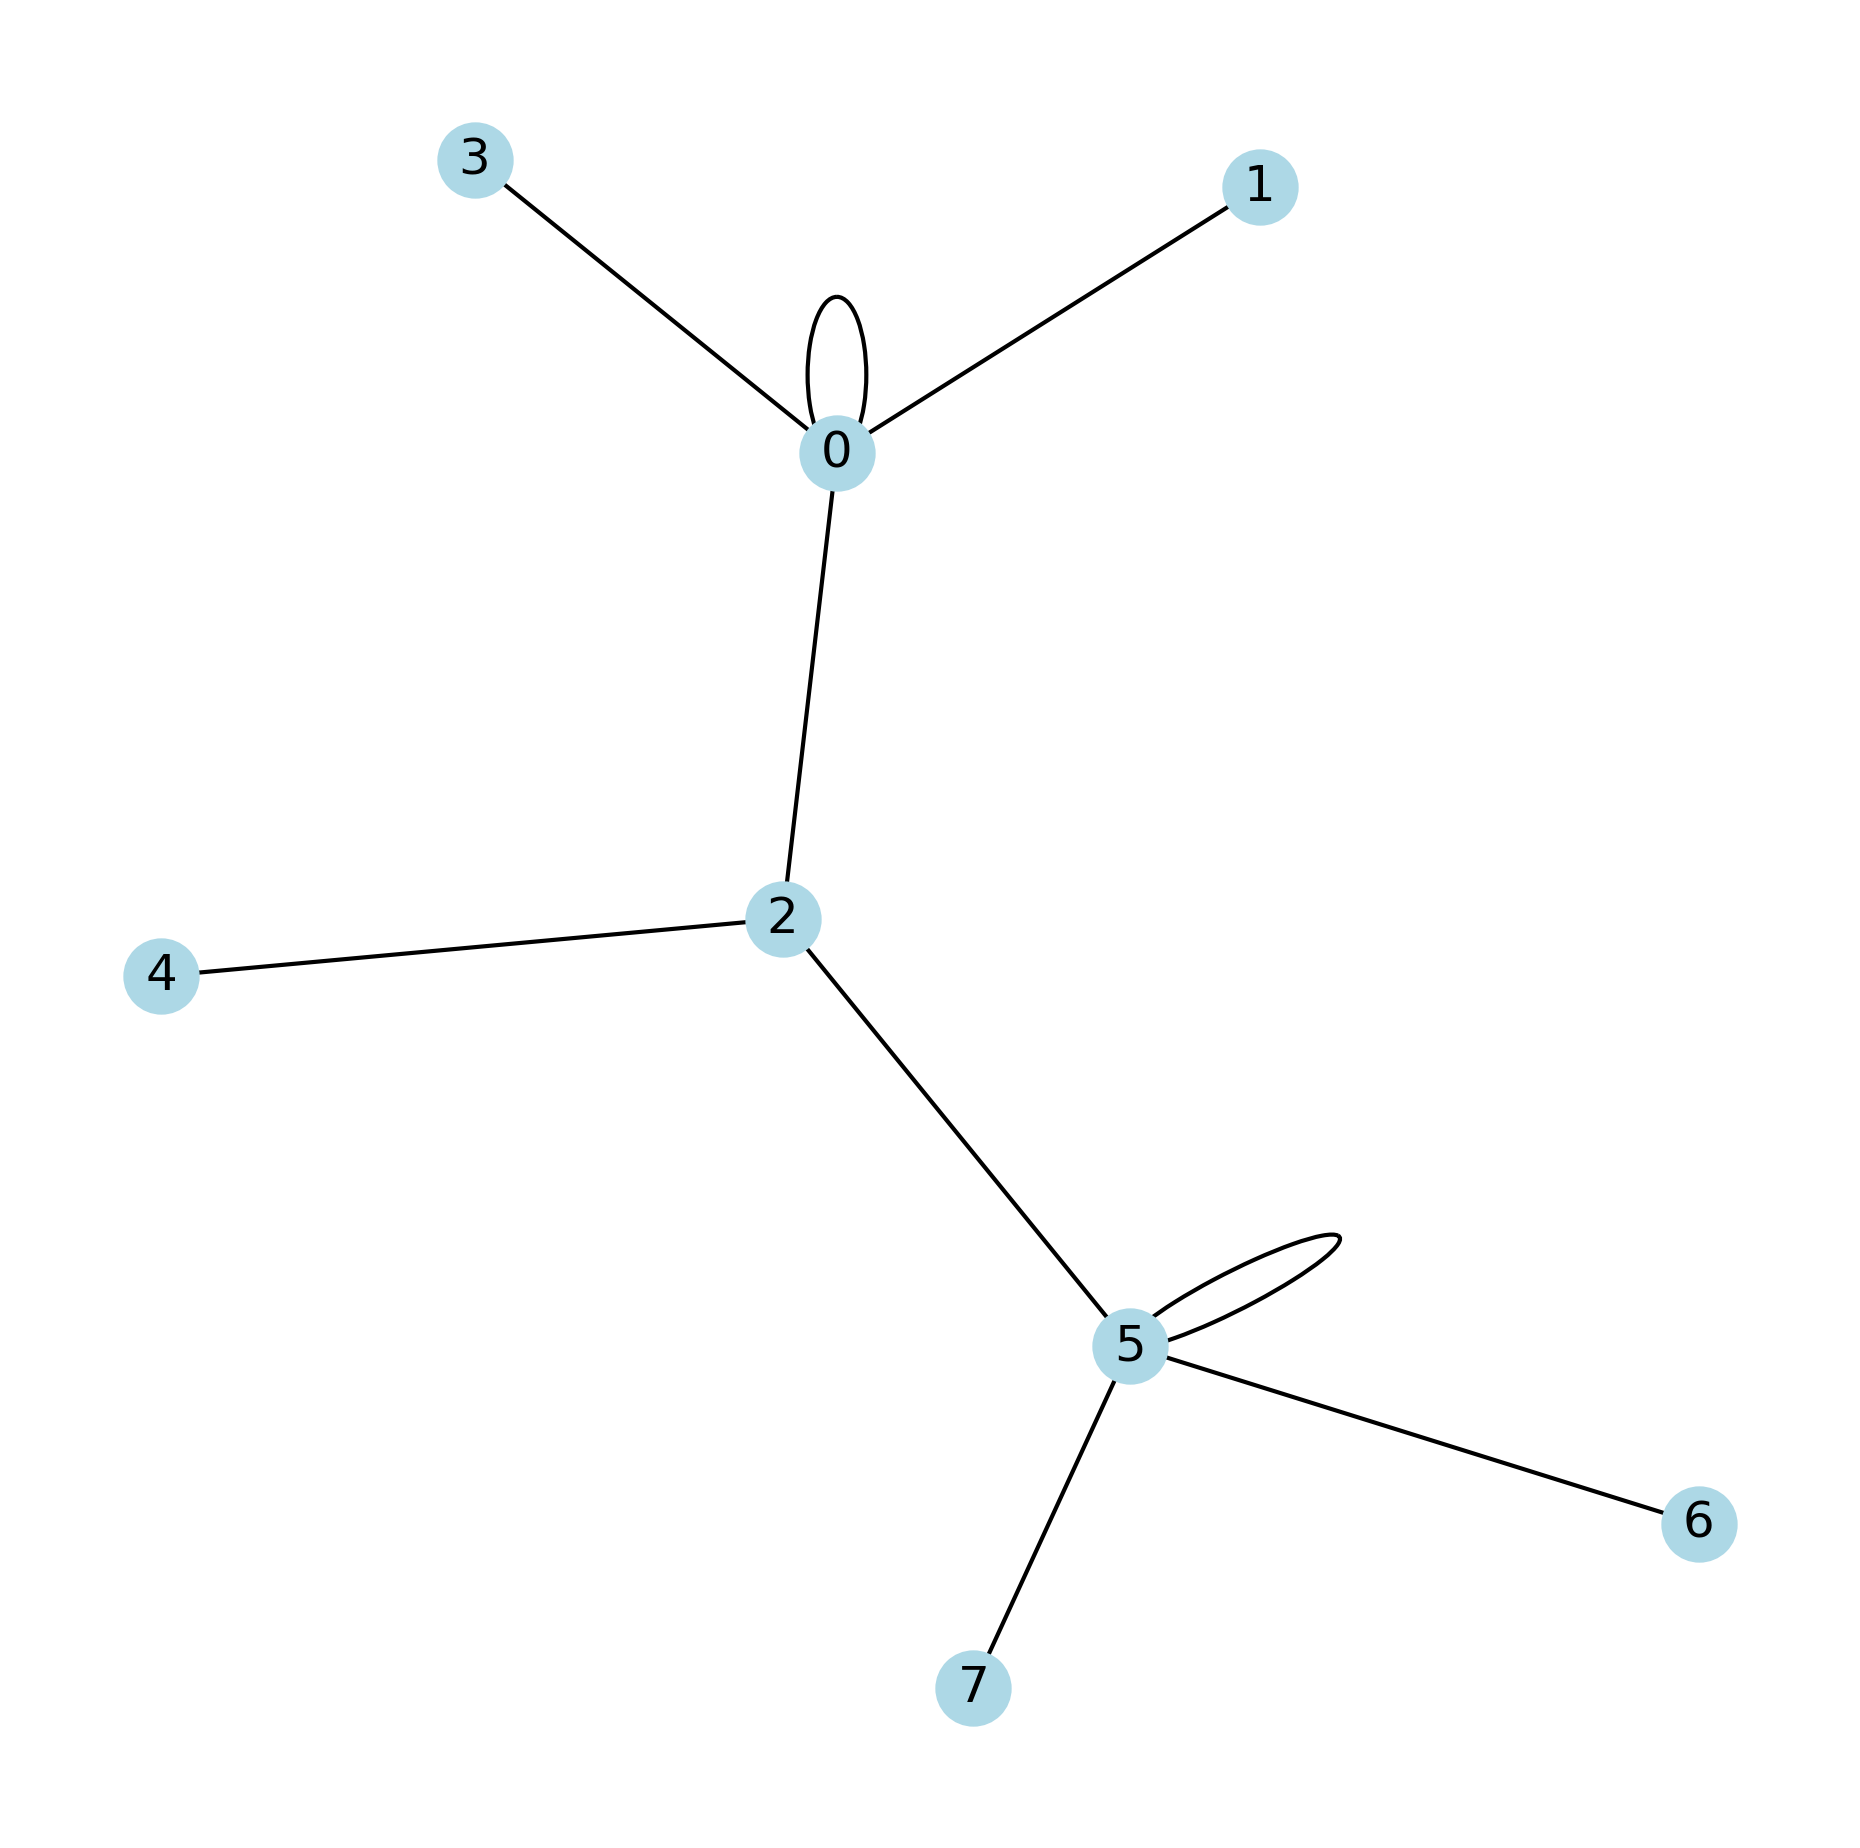
\includegraphics[scale=0.5]{figures/g-004.png}
    \caption{It will become a tree if the loops are removed.}
    \label{fig:4}
\end{figure}

\begin{theorem} \label{thm:3}
    If graph $T$ is loopless and 
	there exists one and only one path 
	connecting each pair of distinct vertices,
	then $T$ is a tree.
\end{theorem}

\begin{proof}
    First, note that $T$ is connected.
	Assume, on the contrary, 
	there exists a cycle $C$ in  $G$.
	Let  $e$ be an edge in  $C$.
	Since  $T$ is assumed loopless, 
	the two ends of  $e$ must be distinct, say  $x$ and $y$.

	Note that there exists a $(x,y)$-path in  $C - e$,
	which is different from the path $xy$. 
	(In fact, this path is $C-e$ itself.) 
	This leads to a contradiction.
\end{proof}

%------------------------------

\begin{theorem} \label{thm:4}
    Let $T$ be a tree. Then we have 
	\begin{align}
		\abs{E} = \abs{V} - 1
		\label{eq:10}
	\end{align}
\end{theorem}

\begin{proof}
	We shall prove by induction on the order $\abs{V}$.

	\noindent\textbf{Base Case:} If $\abs{V} = 1$, 
	then $T$ is a trivial graph without any edges, 
	and hence \eqref{eq:10} holds.

	\noindent\textbf{Inductive Step:} Assume this theorem 
	holds for any trees with order $k$.
	Suppose now $\abs{V(T)} = k+1$.
	Pick a leaf $v$, and then remove it from $T$.
	This is always possible as we have noted.
	Observe that  $T - v$ remains a tree.
	And by removing $v$, 
	we only remove a single edge from  $T$ since  $\deg(v) = 1$.
	Therefore, $\abs{E(T-v)} = \abs{E(T)} - 1$.
	But by the induction hypothesis, 
	we know $\abs{E(T-v)} = \abs{V(T-v)} - 1 = k - 1$. 
	It then follows that 
	 \begin{align*}
		 \abs{E(T)} = \abs{E(T-v)} + 1 
		 = k-1+1
		 = (k+1)-1 
		 = \abs{V(T)} - 1
	\end{align*}
	This completes the proof.
\end{proof}

%------------------------------

\begin{corollary} \label{cor:1}
	Every nontrivial tree has at least two leafs.
\end{corollary}

\begin{proof}
	As we have noted, 
	a nontrivial tree $T$ has at least one leaf.
	Assume $T$ only has one leaf.
	Then we have 
	\begin{align*}
		\sum_{v \in V} \deg(v)
		\geq 1 + 2 (\abs{V} - 1)
		= 2 \abs{V} - 1
	\end{align*}
	since all vertices, except one, 
	are of degree at least 2.
	Combined with Theorem~\ref{thm:5}, we know 
	\begin{align}	
		2\abs{E} = \sum_{v \in V} \deg(v)
		= 2 \abs{V} - 1
		\label{eq:12}
	\end{align}
	On the other hand, it follows from Theorem~\ref{thm:4} that 
	\begin{align}
		2\abs{E} = 2 \abs{V} - 2
		\label{eq:13}
	\end{align}
	Note that equations \eqref{eq:12} and \eqref{eq:13}
	contradict each other. 
	Therefore, $T$ has at least two leafs.
\end{proof}

%------------------------------

\begin{theorem} \label{thm:7}
	Let $T$ be a graph with $\abs{T}-1$ edges, 
	then the following statements are equivalent:
	\begin{enumerate}
		\item $T$ is a tree.
		\item $T$ is connected.
		\item $T$ is acyclic.
	\end{enumerate}
\end{theorem}

\begin{proof}
	Note that we only need to show 2 $\implies$ 3
	and 3 $\implies$ 2.

	(2 $\implies$ 3) By Proposition~\ref{pro:8}, we know
	$T$ is a connected graph with minimum number of edges.
	We need to show $T$ is acyclic.
	Assume that, on the contrary, there exists a cycle $C$ in $T$.
	Pick an edge $e$ in $C$.
	Note that $e$ cannot be a cut edge by Theorem~\ref{thm:6}.
	Therefore, $G-e$ remains connected.
	But clearly $G-e$ has one less edge than that of $G$, 
	which leads to a contradiction.
	Therefore, $T$ is indeed acyclic.

	(3 $\implies$ 2) This direction follows directly 
	from Proposition~\ref{pro:9}.
\end{proof}

%==============================

% references
\printbibliography[heading=bibintoc, title=References]

%==============================

% print index page
\printindex

%==============================

\end{document}
